\documentclass{beamer}
%\documentclass[handout]{beamer}
%\includeonlyframes{current}
\includeonlylecture{week-18}

% Algorithm package with french commands
\usepackage{algcompatible}
\renewcommand{\algorithmicrequire}{\textbf{Entrée :}}
\renewcommand{\algorithmicensure}{\textbf{Sortie :}}
\renewcommand{\algorithmicend}{\textbf{fin}}
\renewcommand{\algorithmicif}{\textbf{si}}
\renewcommand{\algorithmicthen}{\textbf{alors}}
\renewcommand{\algorithmicelse}{\textbf{sinon}}
\newcommand{\algorithmicelsif}{\algorithmicelse\ \algorithmicif}
\newcommand{\algorithmicendif}{\algorithmicend\ \algorithmicif}
\renewcommand{\algorithmicfor}{\textbf{pour}}
\renewcommand{\algorithmicforall}{\textbf{pour chaque}}
\renewcommand{\algorithmicdo}{\textbf{faire}}
\newcommand{\algorithmicendfor}{\algorithmicend\ \algorithmicfor}
\renewcommand{\algorithmicwhile}{\textbf{tant que}}
\newcommand{\algorithmicendwhile}{\algorithmicend\ \algorithmicwhile}
\renewcommand{\algorithmicloop}{\textbf{boucle}}
\newcommand{\algorithmicendloop}{\algorithmicend\ \algorithmicloop}
\renewcommand{\algorithmicrepeat}{\textbf{répète}}
\renewcommand{\algorithmicuntil}{\textbf{jusqu'à}}
\newcommand{\algorithmicprint}{\textbf{affiche}}
\newcommand{\algorithmicreturn}{\textbf{retourne}}
\newcommand{\RETURN}{\STATE \algorithmicreturn \ }
\newcommand{\algorithmictrue}{\textbf{vrai}}
\newcommand{\algorithmicfalse}{\textbf{faux}}

\usetheme{Antibes}

\definecolor{GyBusPurple}{HTML}{464883} % GyBus Hexa colors

\usecolortheme[named=GyBusPurple]{structure}

\title{Informatique 1M3}
\subtitle{Enseignement obligatoire de l'informatique au gymnase}
\author{Tom Demont}
\date{2022-2023}
\institute{Gymnase de Bussigny}

\begin{document}

\AtBeginSection {
	\begin{frame}{Plan}
		\tableofcontents[
			currentsection,
			hideallsubsections
		]
	\end{frame}
}

\AtBeginSubsection {
	\begin{frame}{Plan}
		\tableofcontents[
			sectionstyle=show/hide,
			subsectionstyle=show/shaded/hide
		]
	\end{frame}
}

\lecture{Introduction}{week-0}

\begin{frame}
	\titlepage
\end{frame}

\begin{frame}{Table des matières}
	\tableofcontents[hideallsubsections]
\end{frame}

\section{Représentation de l'information}
\subsection{Les entiers}
\subsection{Les caractères}
\subsection{Les images}

\lecture{Taille d'image, compression et images vectorielles}{week-10}

\begin{frame}{Retour sur la séance précédente}{Images en couleur, dimension et résolution}
	\begin{columns}
		\begin{column}{0.6\textwidth}
			\begin{description}
				\item[Couleurs] : chaque pixel est représenté avec 3 nombres $(Red, Green, Blue)$
					\item<2->[Dimension] : le nombre de pixels d'une image numérique
					\item<3->[Résolution] : La densité de pixel par $pouce^{2}$
			\end{description}
		\end{column}
		\begin{column}{0.4\textwidth}
			\begin{figure}
				\includegraphics<2->[width=1\linewidth]{dimension-image.jpg}
			\end{figure}
			\begin{figure}
				
\includegraphics[width=1\linewidth]{binaire-pixel-couleur.jpeg}
			\end{figure}
		\end{column}
	\end{columns}
\end{frame}

\begin{frame}{Calcul de taille d'image}{}
	\begin{alertblock}{Exercice}
		En considérant qu'un pixel en niveau de gris occupe \textbf{1 octet} en mémoire, et qu'un pixel en couleur en occupe \textbf{3}, donnez pour chaque dimension d'image la taille mémoire occupée. En bonus, vous pouvez effectuer la conversion pour les plus grandes images et pour les images en noir et blanc (\textbf{1 bit par pixel})
	\end{alertblock}

	\begin{columns}
		\begin{column}{0.6\textwidth}
			\begin{table}
				\begin{tabular}{| c | c | c || c |}
					\hline
					Définition       & gris & couleur & NB \\
					\hline \hline
					$320\times 200$  &      &         &    \\
					$640\times 480$  &      &         &    \\
					$800\times 600$  &      &         &    \\
					\hline
					Bonus            &      &         &    \\
					$1024\times 768$ &      &         &    \\
					\hline
				\end{tabular}
			\end{table}
		\end{column}
		\begin{column}{0.4\textwidth}
			\begin{figure}
				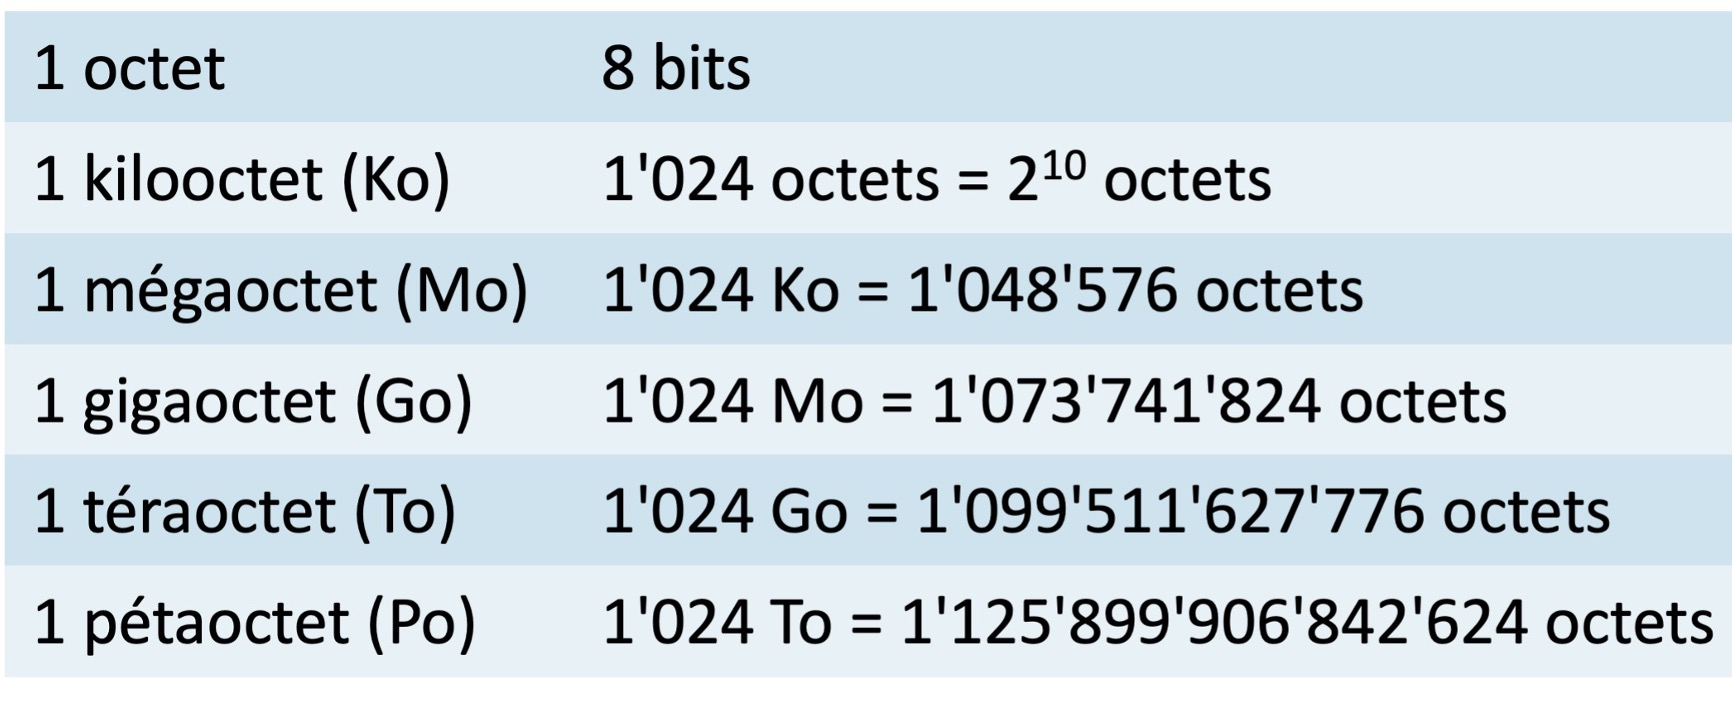
\includegraphics[width=1\linewidth]{conversion-octets.jpg}
			\end{figure}
		\end{column}
	\end{columns}
\end{frame}

\begin{frame}{Calcul de taille d'image}{Solution}
	\begin{exampleblock}{Solution}
		\begin{table}
			\begin{tabular}{| c | c | c || c |}
				\hline
				Définition       & gris      & couleur   & NB       \\
				\hline \hline
				$320\times 200$  & $62.5Ko$  & $187.5Ko$ & $7.8Ko$  \\
				$640\times 480$  & $300Ko$   & $900Ko$   & $37.5Ko$ \\
				$800\times 600$  & $468.7Ko$ & $1.4Mo$   & $58.6Ko$ \\
				\hline
				Bonus            &           &           &          \\
				$1024\times 768$ & $768Ko$   & $2.3Mo$   & $96Ko$   \\
				\hline
			\end{tabular}
		\end{table}
	\end{exampleblock}
	\begin{columns}
		\begin{column}{0.65\textwidth}
			Que signifie qu'un image fasse 2.3Mo ? Combien pouvez vous en mettre sur un téléphone de 32Go ? \uncover<2->{$\frac{32*1024}{2.3}=14246$ photos}
		\end{column}
		\begin{column}{0.35\textwidth}
			\begin{figure}
				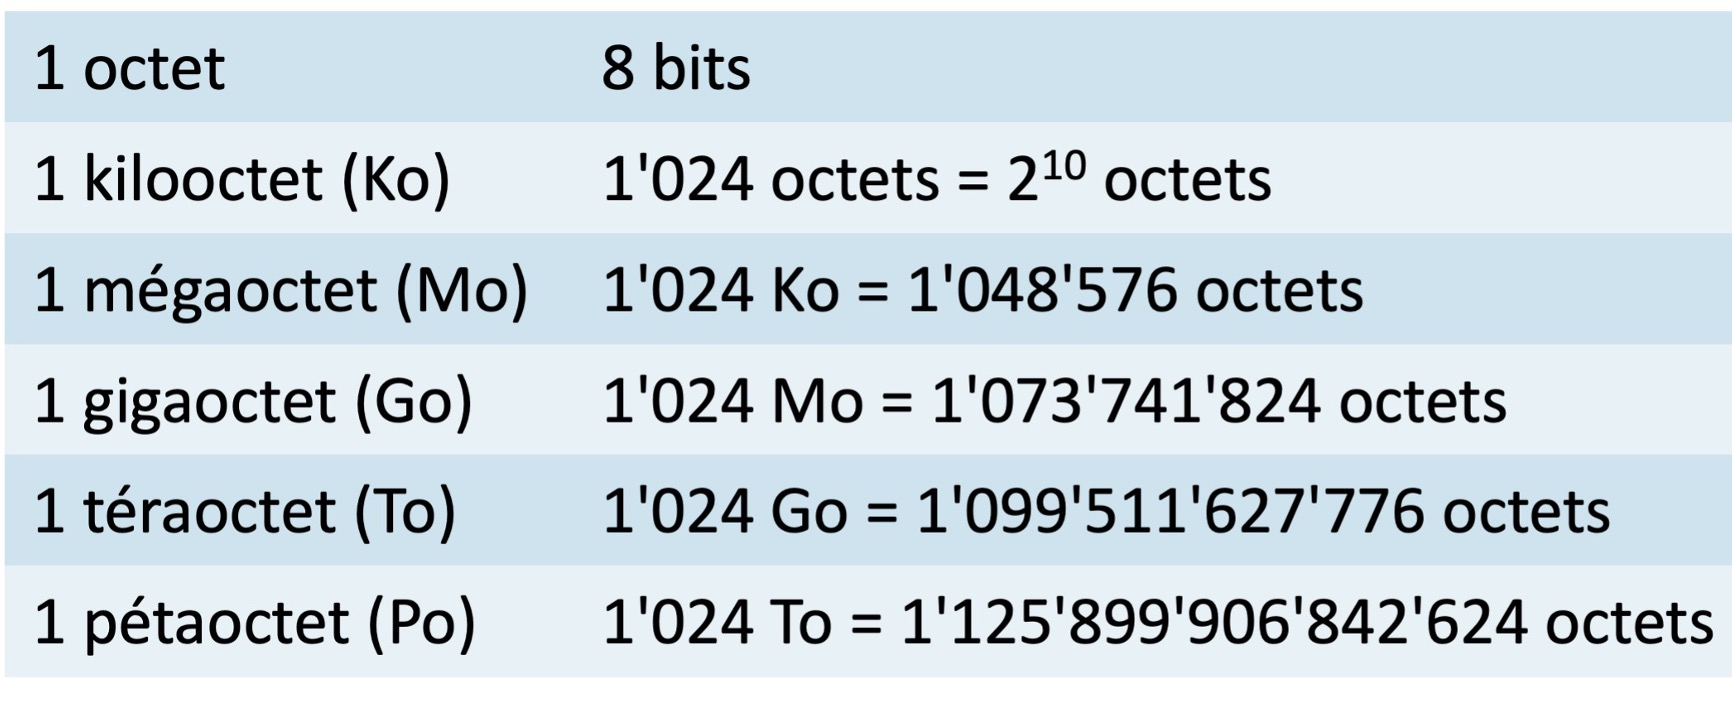
\includegraphics[width=1\linewidth]{conversion-octets.jpg}
			\end{figure}
		\end{column}
	\end{columns}
\end{frame}

\begin{frame}{Compression}{}
	\begin{itemize}
		\item <1->Avez vous déjà entendu parlé de compression ?
		\item <2->Quelle est la différence entre ces deux images :
	\end{itemize}

	\begin{columns}
		\begin{column}{0.5\textwidth}
			\begin{figure}
				\includegraphics<2->[width=0.8\linewidth]{cat.png}
				\uncover<3->{\caption{Compression PNG}}
			\end{figure}
		\end{column}
		\begin{column}{0.5\textwidth}
			\begin{figure}
				\includegraphics<2->[width=0.8\linewidth]{cat.jpeg}
				\uncover<3->{\caption{Compression JPG}}
			\end{figure}
		\end{column}
	\end{columns}
\end{frame}

\begin{frame}{Compression}{PNG et JPG (ou JPEG)}
	\begin{columns}
		\begin{column}{0.5\textwidth}
			\begin{figure}
				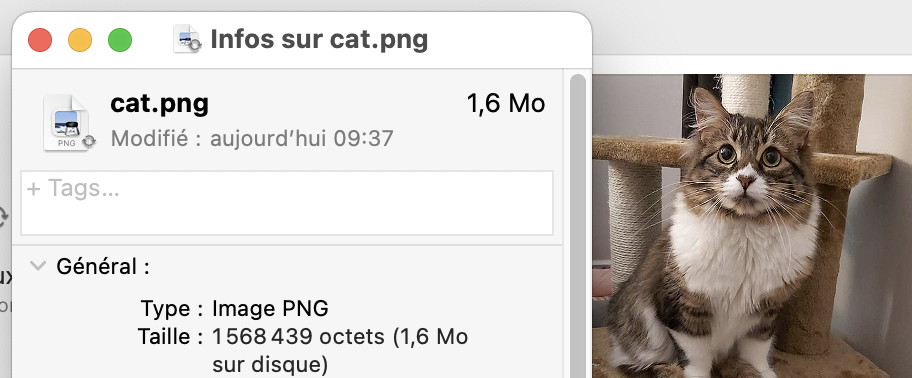
\includegraphics[width=1\linewidth]{cat-png-compression.png}
				\caption{Compression PNG}
			\end{figure}
		\end{column}
		\begin{column}{0.5\textwidth}
			\begin{figure}
				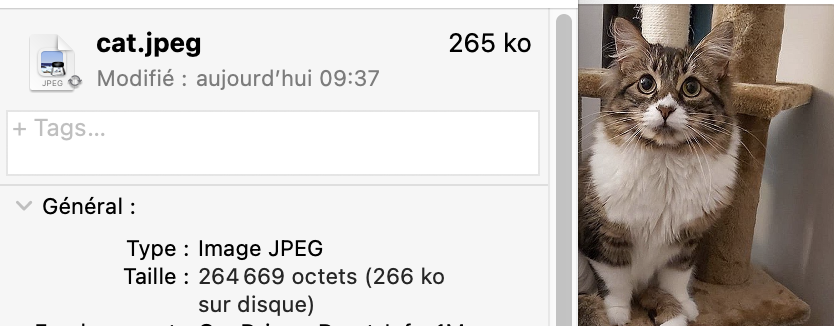
\includegraphics[width=1\linewidth]{cat-jpg-compression.png}
				\caption{Compression JPG (ou JPEG)}
			\end{figure}
		\end{column}
	\end{columns}
\end{frame}

\begin{frame}{Compression}{Différents type de compression}
	\begin{definition}
		\textbf<1,3->{Compression sans perte} : l’image comprimée est parfaitement identique à l’originale. Par exemple, l'algorithme de compression PNG.
	\end{definition}
	\begin{definition}
		\textbf<2->{Compression avec perte} : l’image est plus ou moins dégradée, selon le taux de compression souhaité. Par exemple, l'algorithme de compression JPEG.
	\end{definition}

	\uncover<3->{\href{https://youtu.be/l9yCIbvD2S0?t=1294}{\beamergotobutton{C'est pas Sorcier, algorithmes de compression}}}
\end{frame}

\begin{frame}{Compression et taille}{Compression avec perte et taux de compression}
	\begin{block}{Taux de compression}
		Le taux de compression détermine à quel point la taille d'un fichier peut être réduite par notre algorithme de compression. Il se calcule comme : $1-\frac{\text{taille du fichier compressé}}{\text{taille du fichier sans compression}}$
	\end{block}

	\uncover<2->{\begin{exampleblock}{Exemple}
			Considérons image en niveau de gris de 1024 pixels. Elle a donc une taille non compressée de 1Ko. On nous dit que cette image compressée a une taille de 256 octets. Son taux de compression est donc $1-\frac{256}{1024}=1-\frac{1}{4}=75\%$
		\end{exampleblock}}
\end{frame}

\begin{frame}{Compression et taille}{}
	\begin{alertblock}{Exercice}
		Une image \textbf{niveaux de gris} de format 1024 X 1024 est enregistrée en JPG. Le taux de compression est de 50\%. Quelle est sa taille sur le disque dur (détaillez les calculs) ?
	\end{alertblock}
	\uncover<2->{\begin{exampleblock}{Solution}
			On multiplie 1024 x 1024 = 1048576 : c’est le nombre de pixels et la taille initiale de l’image en octets puisque l’image est en niveaux de gris (codage 1 octet). Comme le taux de compression est 50\%, on a $1-\frac{\text{taille du fichier compressé}}{\text{taille du fichier sans compression}}=\frac{1}{2}$\\$ \leftrightarrow \text{taille du fichier compressé}=\frac{\text{taille du fichier sans compression}}{2}=524288\ octets=512Ko$.
		\end{exampleblock}}
\end{frame}

\begin{frame}{Images vectorielles}{}
	\begin{block}{Principe}
		Au lieu de stocker chaque pixels d'une image (limité par une certaine dimension d'image définie), on enregistre des objets géométriques (cercles, traits, courbes).
	\end{block}

	\begin{columns}
		\begin{column}{0.5\textwidth}
			\begin{exampleblock}{Avantages}
				\begin{itemize}
					\item Permet de stocker des images de la taille voulue (ne dépend pas de la dimension)
					\item ``Zoomer à l'infini'', car les images sont agrandies avec des calculs sur les formes géométriques
				\end{itemize}
			\end{exampleblock}
		\end{column}
		\begin{column}{0.5\textwidth}
			\begin{alertblock}{Inconvénients}
				\begin{itemize}
					\item Limite de réalisme : dur de tout représenter par des formes géométriques simples
					\item Nécessite des logiciels spéciaux (Adobe InDesign, Inkscape)
				\end{itemize}
			\end{alertblock}
		\end{column}
	\end{columns}
\end{frame}

\begin{frame}{Images vectorielles}{}
	\begin{alertblock}{Exercice}
		Décidez quelle image est stockée sous forme vectorielle et laquelle est stockée sous forme matricielle.
	\end{alertblock}
	\begin{figure}
		
\includegraphics[width=0.7\linewidth]{matvect.png}
		\uncover<2->{\caption{Gauche : vectoriel, droite : matriciel}}
	\end{figure}
\end{frame}

\lecture{Le son}{week-12}

\subsection{Le son}

\begin{frame}{Le son}{Un phénomène physique}
	\begin{definition}
		Le son est une \textbf{onde mécanique} qui se propage dans l'air. L'amplitude et la fréquence permettent de définir différents types de sons.
	\end{definition}
	\begin{columns}
		\begin{column}{0.5\textwidth}
			\textbf{Amplitude} : à quel point l'air vibre fort.
			\begin{figure}
				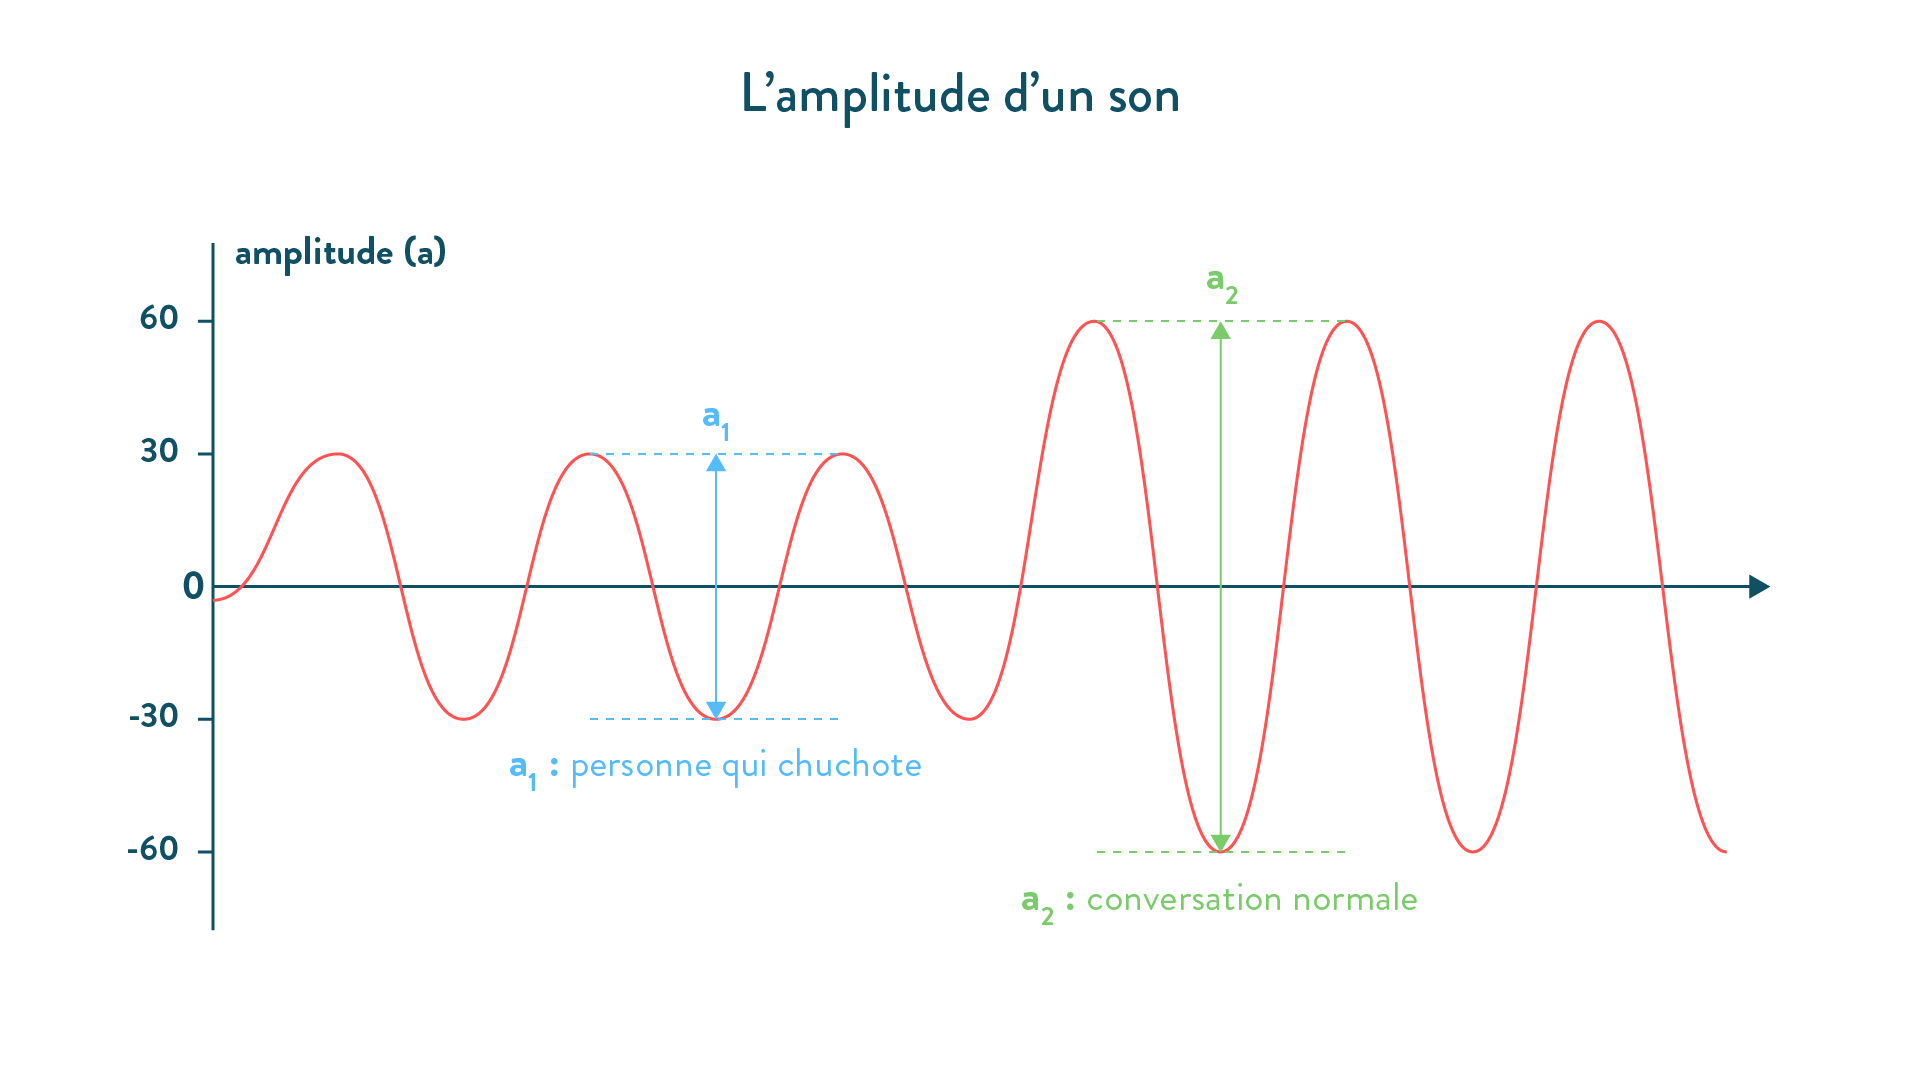
\includegraphics[width=1\linewidth]{amplitude-son.png}
			\end{figure}
		\end{column}
		\begin{column}{0.5\textwidth}
			\textbf{Fréquence} : à quel point l'air vibre vite.
			\begin{figure}
				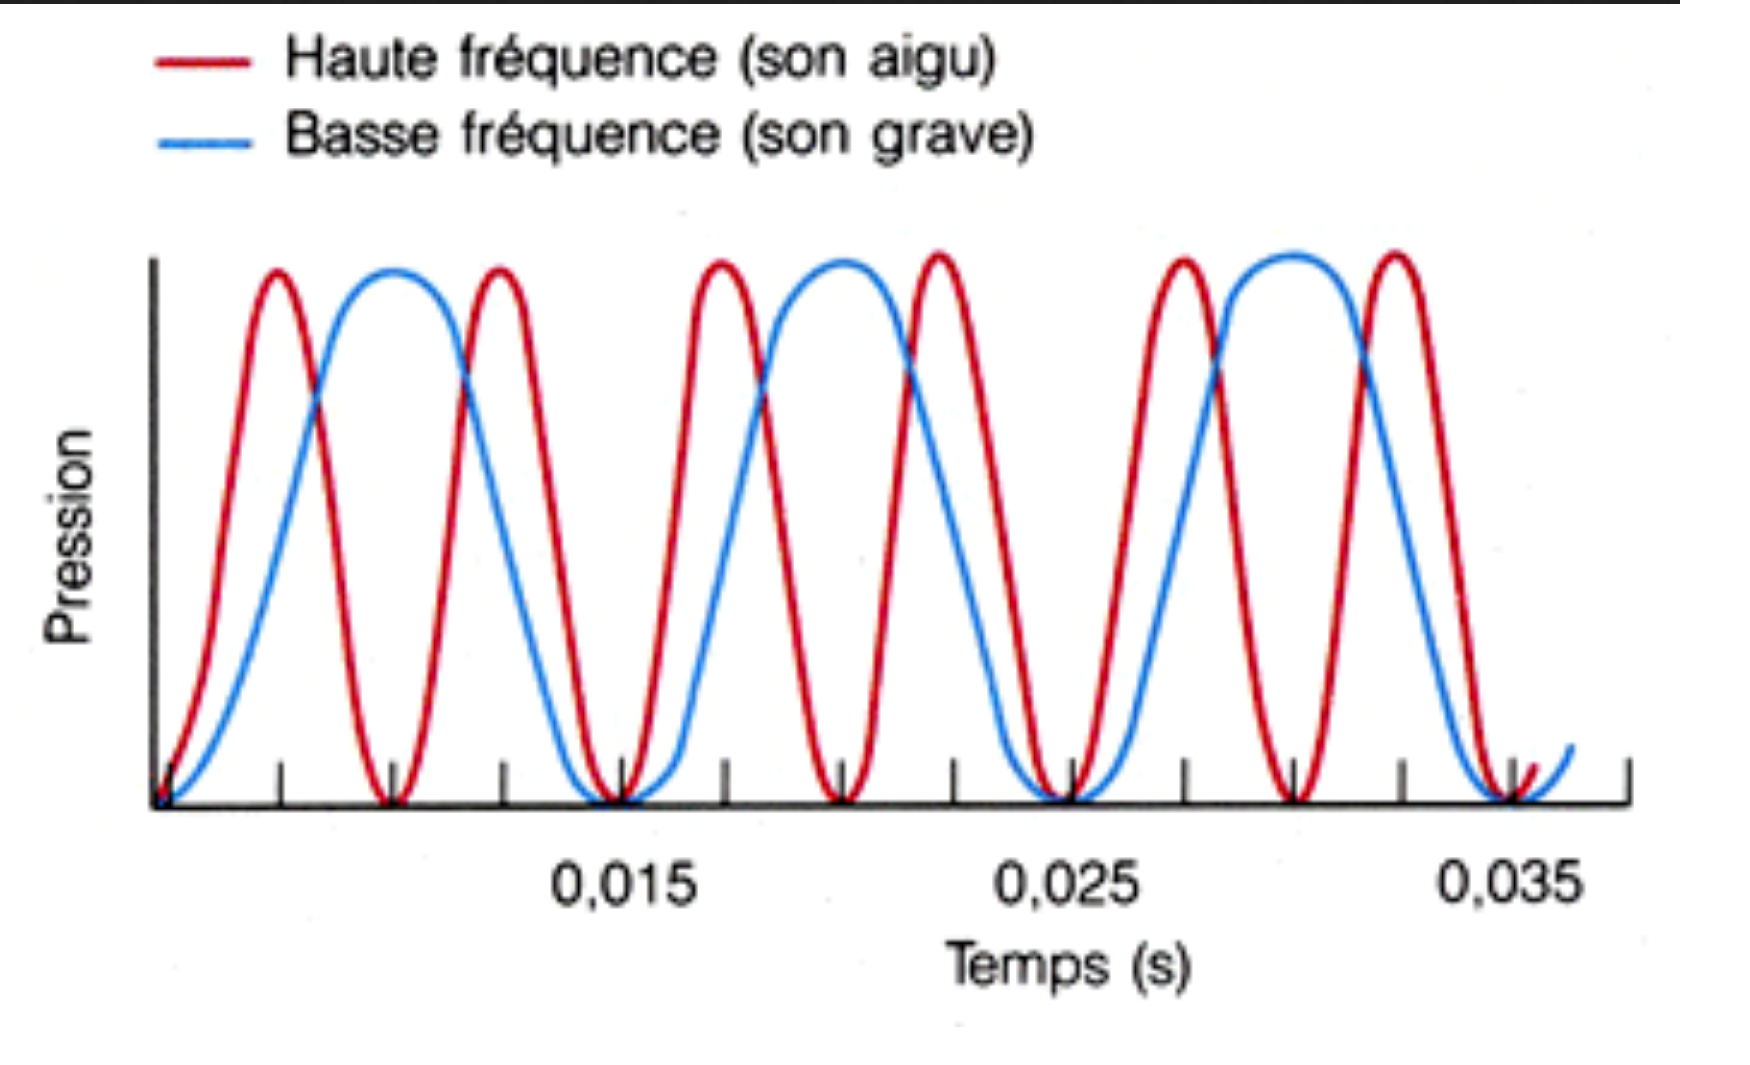
\includegraphics[width=0.85\linewidth]{frequence-son.png}
			\end{figure}
		\end{column}
	\end{columns}
\end{frame}

\begin{frame}{Transmission du son}{Voix et oreilles}
	\begin{figure}
		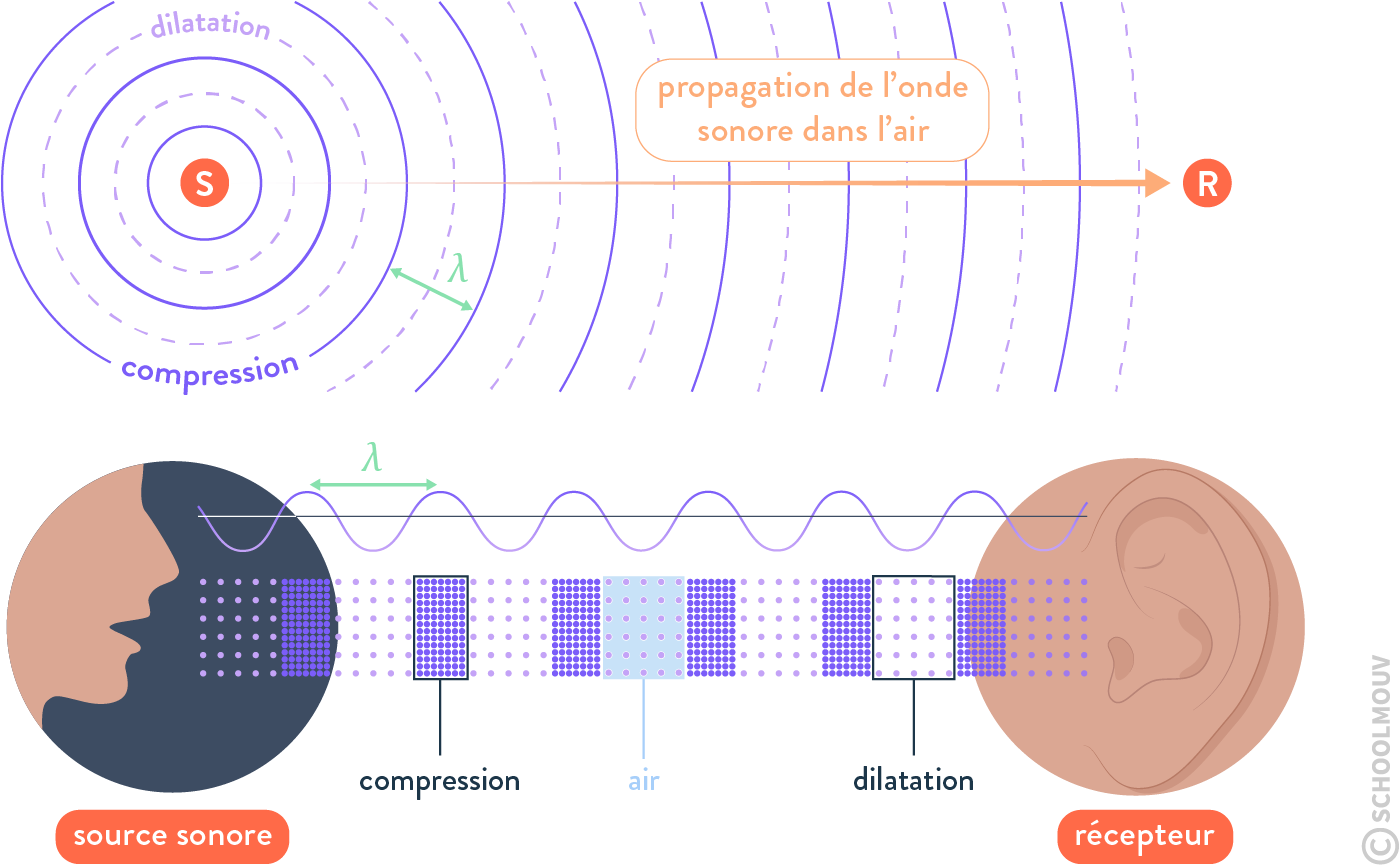
\includegraphics[width=0.65\linewidth]{transmission-son.png}
	\end{figure}
	\href{https://youtu.be/QEpk6feHMxQ}{\beamergotobutton{2 minutes pour comprendre : le son}}
\end{frame}

\begin{frame}{Transmission du son}{}

	\begin{alertblock}{Exercice}
		Complétez les schémas distribués en y ajoutant les étapes allant de la création du son produit par un.e humain.e, jusqu'à la compréhension de ce son par un.e autre humain.e.
	\end{alertblock}

\end{frame}

\begin{frame}{Transmission du son}{}
	\begin{exampleblock}{Solution}
		\begin{figure}
			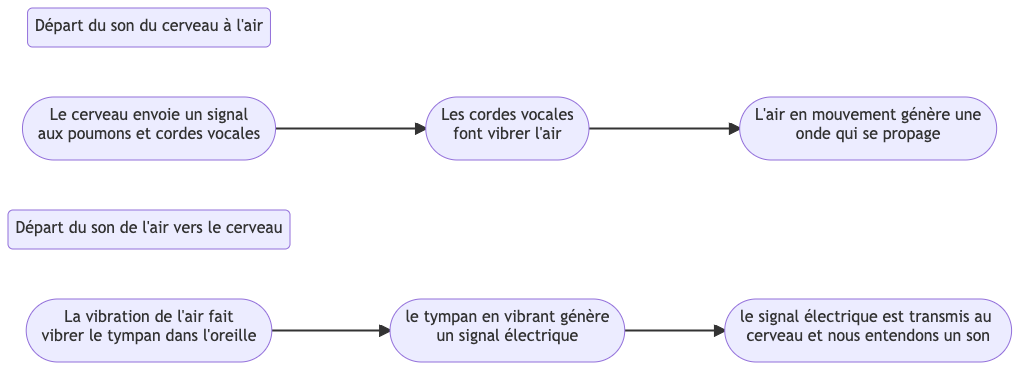
\includegraphics[width=1\linewidth]{solution-transmission-son.png}
		\end{figure}
	\end{exampleblock}

\end{frame}

\begin{frame}{Le son : une onde continue}{}
	\begin{itemize}
		\item Le son est une onde \textbf{continue}
		\item Impossible de représenter infiniment précisément la position des atomes propageant l'onde
		\item Choisir seulement certains moments à capturer
	\end{itemize}
	\uncover<2->{\begin{figure}
			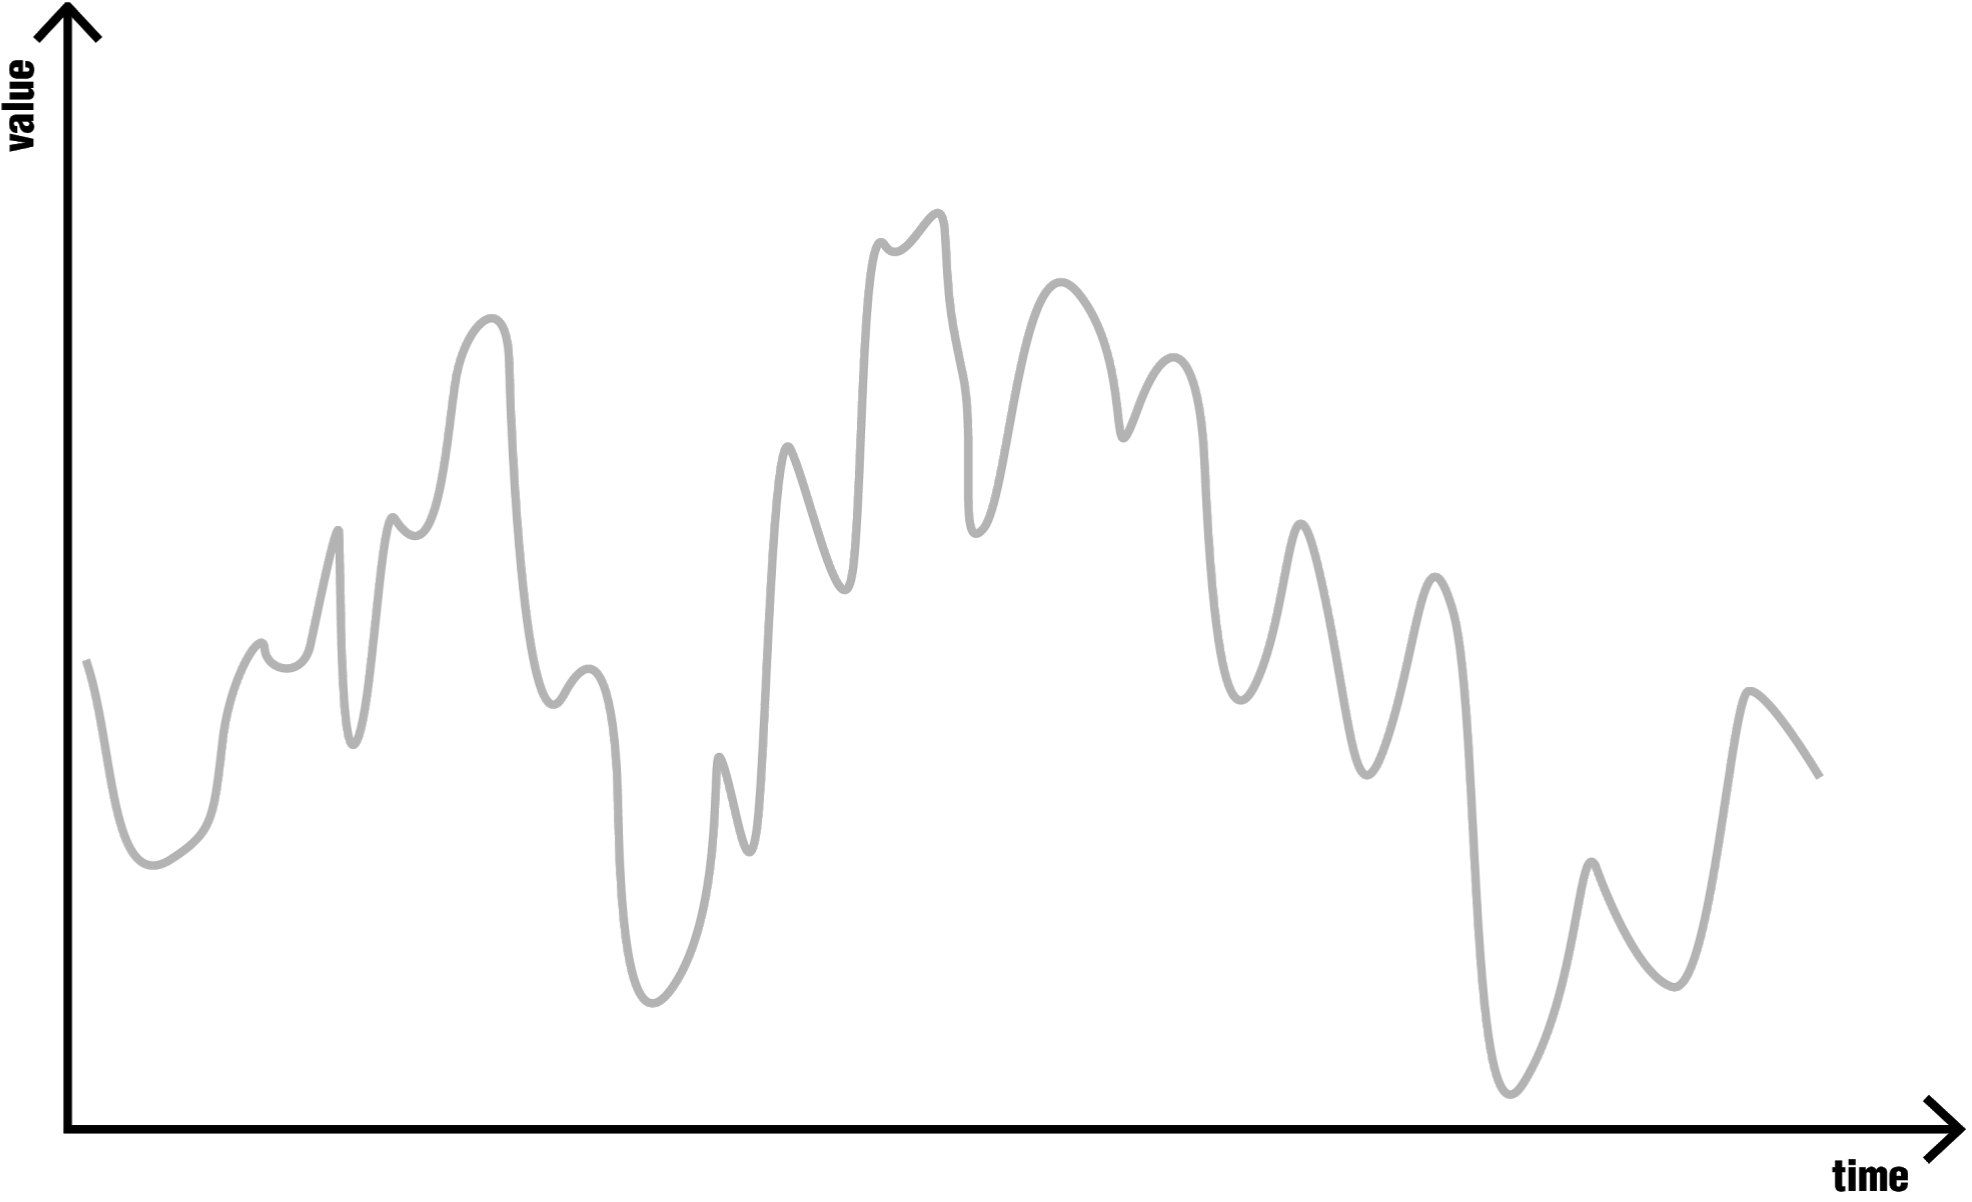
\includegraphics[width=0.5\linewidth]{soncontinu.png}
			\caption{Exemple de représentation d'une onde sonore}
		\end{figure}}
\end{frame}

\begin{frame}{Convertir le son}{Processus en 3 étapes}

	\begin{itemize}
		\item<1-> Échantillonnage
		\item<2-> Quantification
		\item<3-> Encodage
	\end{itemize}

\end{frame}

\begin{frame}{Echantillonnage}{Sélectionner les moments à capturer}
	\begin{definition}
		Fréquence d'échantillonnage : intervalle temporel entre deux mesures de notre onde.
	\end{definition}
	\begin{figure}
		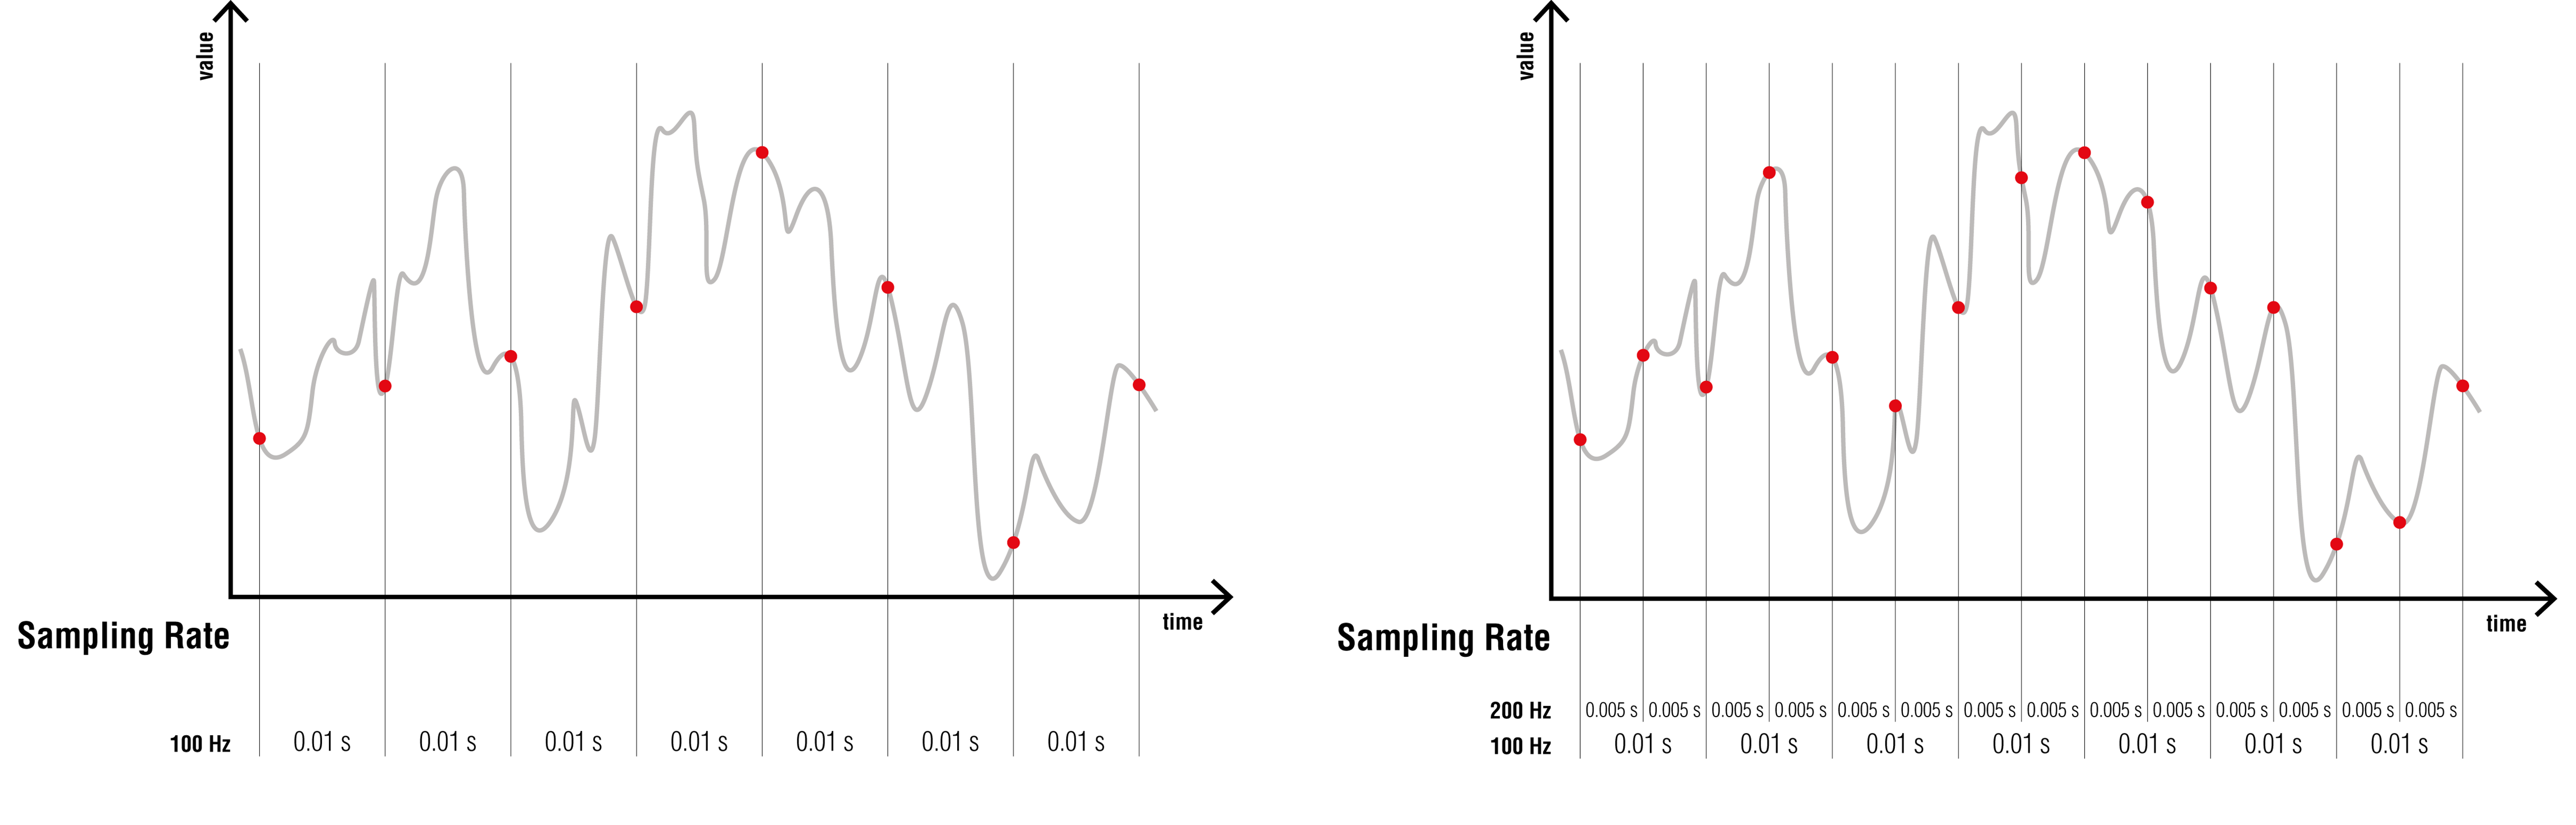
\includegraphics[width=1\linewidth]{numerisation-01.png}
		\caption{Onde capturée avec différentes fréquences d'échantillonnage. Seuls les points rouge sont conservés dans la mémoire.}
	\end{figure}

\end{frame}

\begin{frame}{Echantillonnage}{}
	\begin{block}{Compromis de l'échantillonnage}
		Une plus grande fréquence d'échantillonnage permet de restituer un son de meilleur qualité, mais demande de stocker plus de points de capture en mémoire.
	\end{block}
	\href{https://youtu.be/6kIHsGJSUrY?t=91}{\beamergotobutton{Différentes qualités de son à différentes fréquences d'échantillonnage}}
\end{frame}

\begin{frame}{Quantification}{Taille des échantillons de capture}
	On sait combien d'échantillons capturer. Mais combien de bits utiliser pour représenter chaque échantillon ?
	\begin{definition}
		Quantification : choix du nombre de bits utilisés pour représenter un échantillon. Définit la précision d'un échantillon.
	\end{definition}
	\uncover<2->{\begin{figure}
			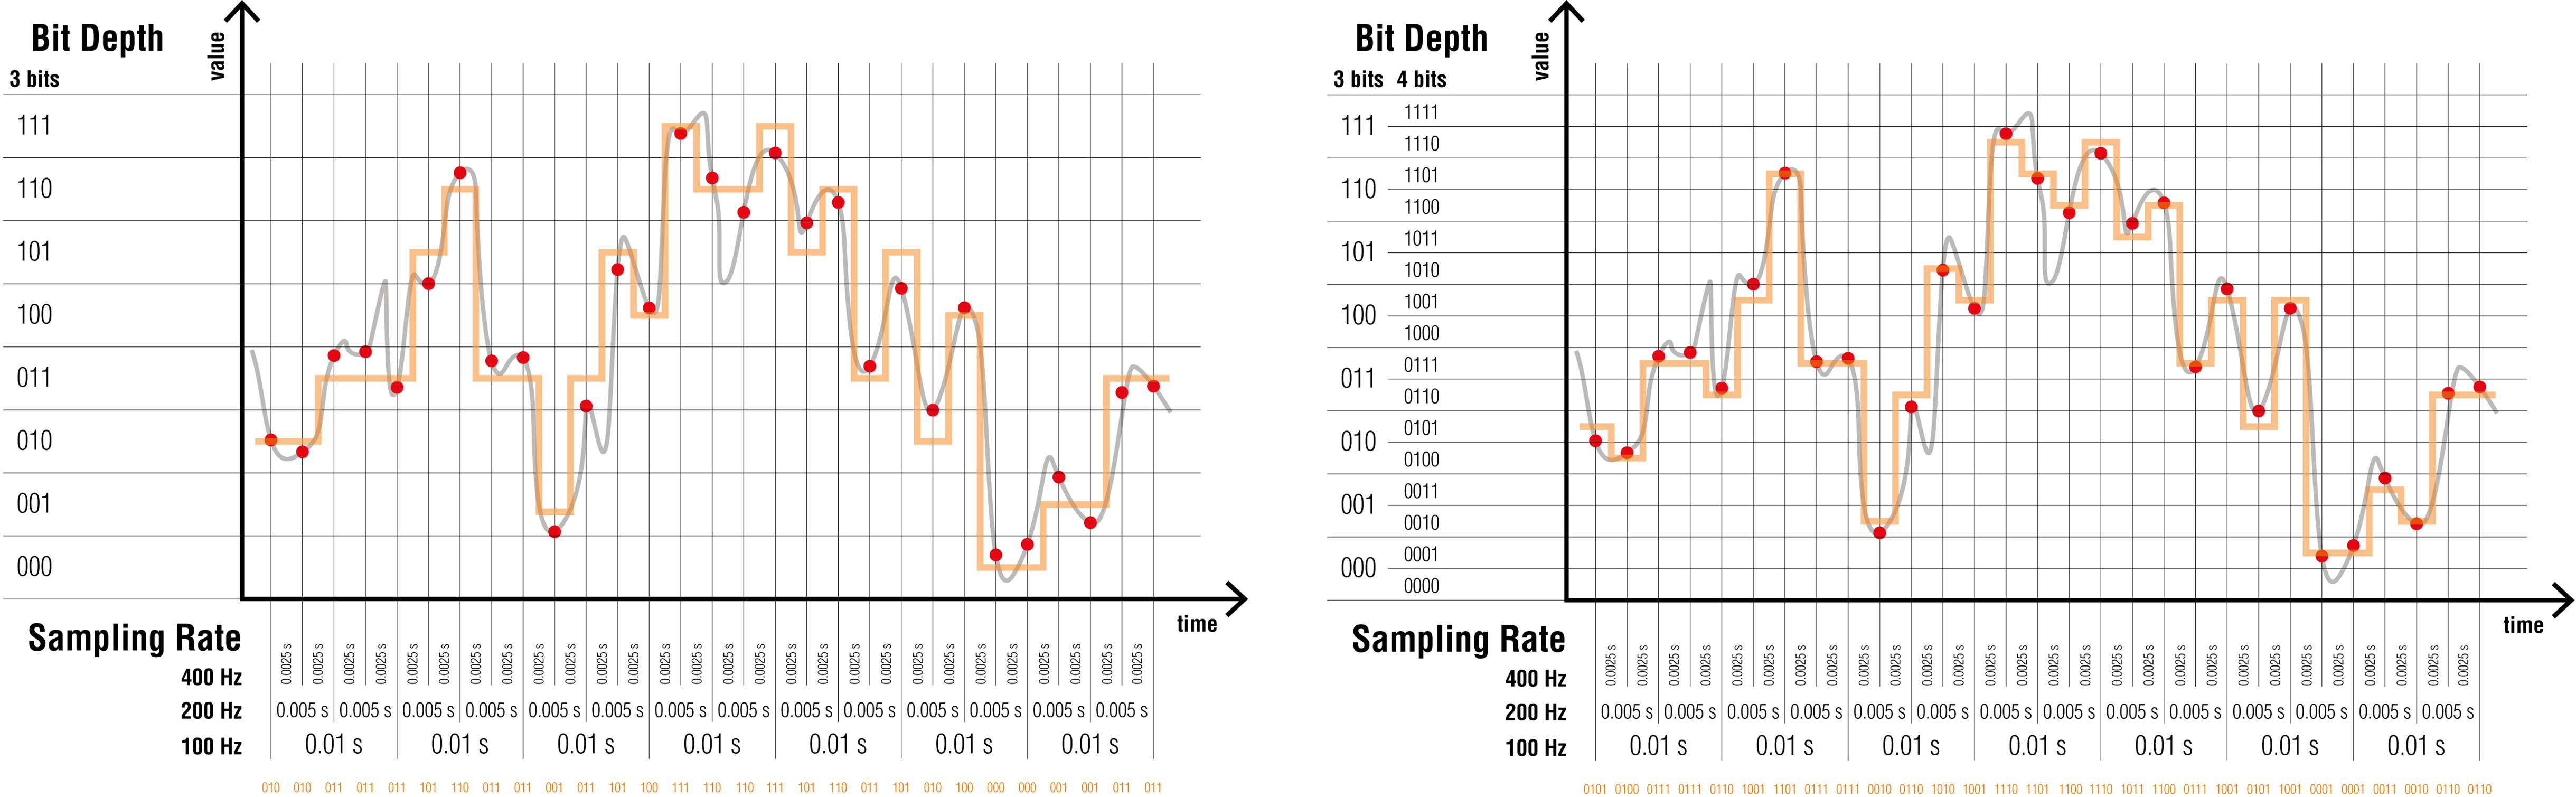
\includegraphics[width=0.9\linewidth]{numerisation-02.png}
			\caption{Onde capturée avec différentes profondeur d'échantillonnage}
		\end{figure}}
\end{frame}

\begin{frame}{Quantification}{}
	\begin{block}{Compromis de la quantification}
		Une plus grande profondeur d'échantillonnage permet de restituer un son de meilleur qualité, mais demande de stocker des points de capture plus gros en mémoire.
	\end{block}
	\href{https://youtu.be/6kIHsGJSUrY}{\beamergotobutton{Différentes qualités de son à différentes profondeurs d'échantillonnage}}
\end{frame}

\begin{frame}{Encodage}{Mettre tout le monde d'accord sur la représentation de ces échantillons}
	Dernière étape : encodage.
	\begin{itemize}
		\item Différents formats existent (MP3, flac, AAC, etc.).
		\item Certains optimisent la mémoire (moins d'espace pour stocker le son)
		\item D'autres optimisent la reconstruction (plus facilement pour l'ordinateur de produire le son à partir du fichier).
	\end{itemize}
\end{frame}

\begin{frame}{Exercice}{Numérisation d'un signal sonore}
	\begin{alertblock}{Exercice}
		Complétez le document distribué en indiquant les échantillons stockés en mémoire selon différents paramètres. A finir à la maison.
	\end{alertblock}
\end{frame}

\begin{frame}{Exercice}{Numérisation d'un signal sonore}
	\begin{exampleblock}{Solution}
		On dessine une ``grille'' déterminant les possibles points de numérisation : une colonne toutes les 0.0025 secondes pour 400Hz et une toutes les 0.005 secondes pour 200Hz. Pour les lignes, on en dessiner $2^{4}=16$ pour 4 bits et $2^{3}=8$ pour 8 bits. On s'occupe ensuite d'approximer le passage de la courbe aux coins de cette grille : ce sont les points que l'on va stocker numériquement.
	\end{exampleblock}

\end{frame}
\begin{frame}{Exercice}{Numérisation d'un signal sonore}
	\begin{figure}
		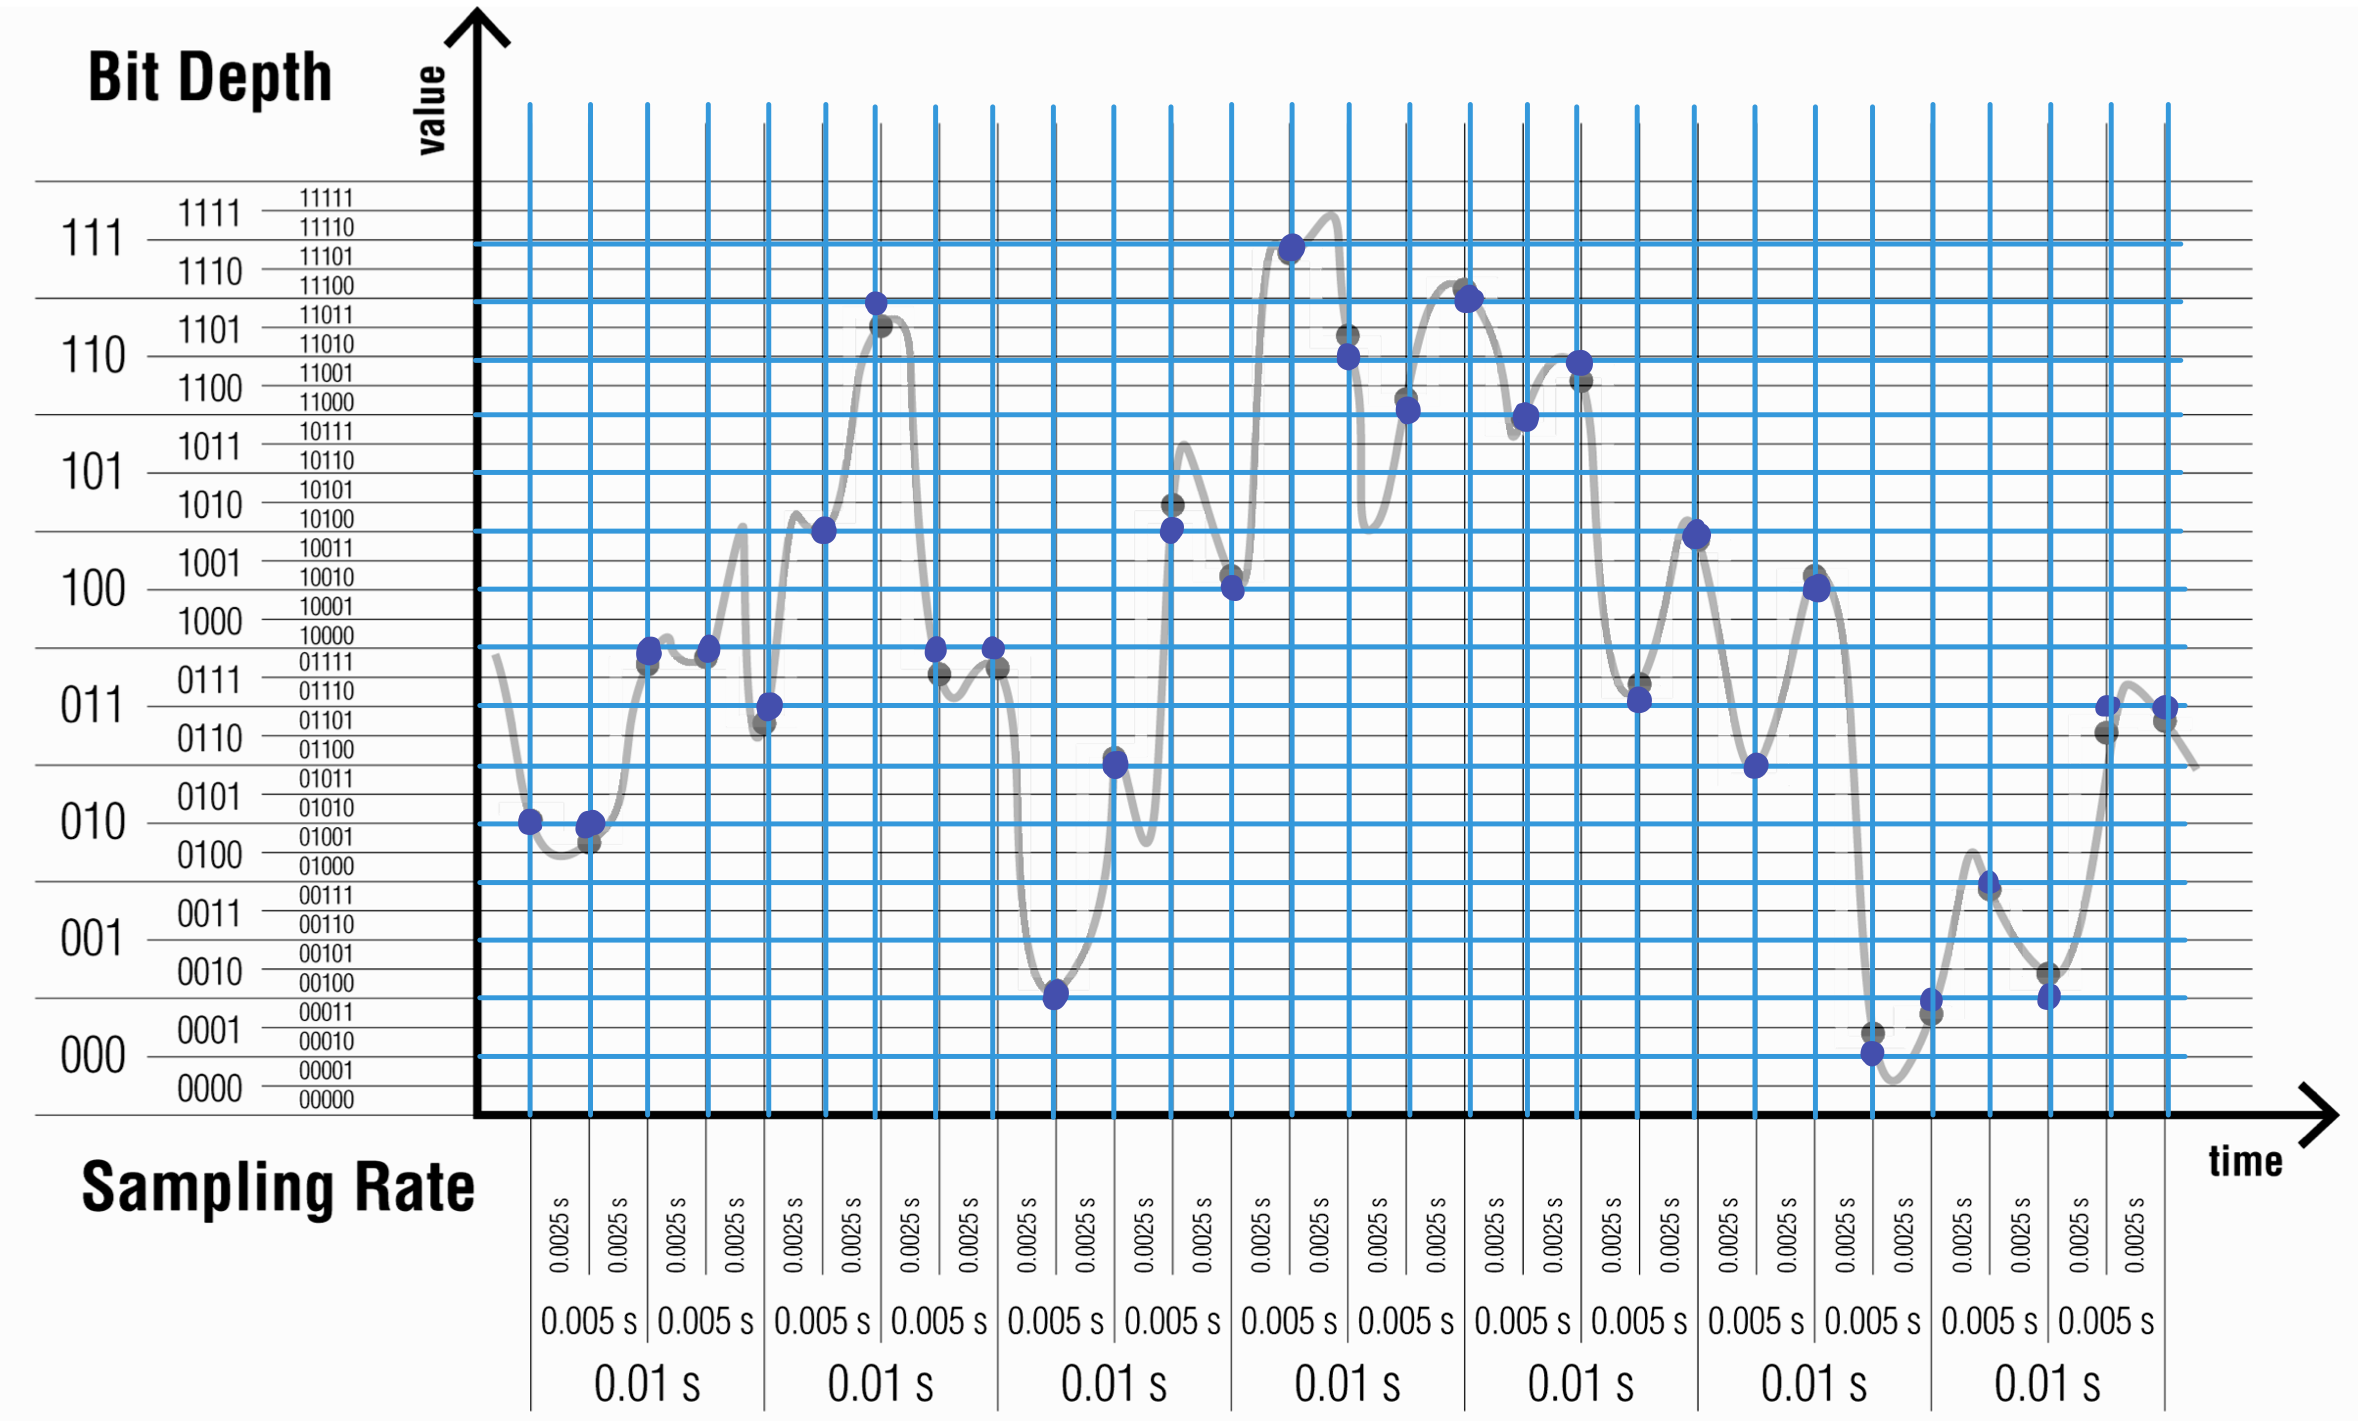
\includegraphics[width=1\linewidth]{solution-sampling-1.png}
	\end{figure}
\end{frame}

\begin{frame}{Exercice}{Numérisation d'un signal sonore}
	\begin{figure}
		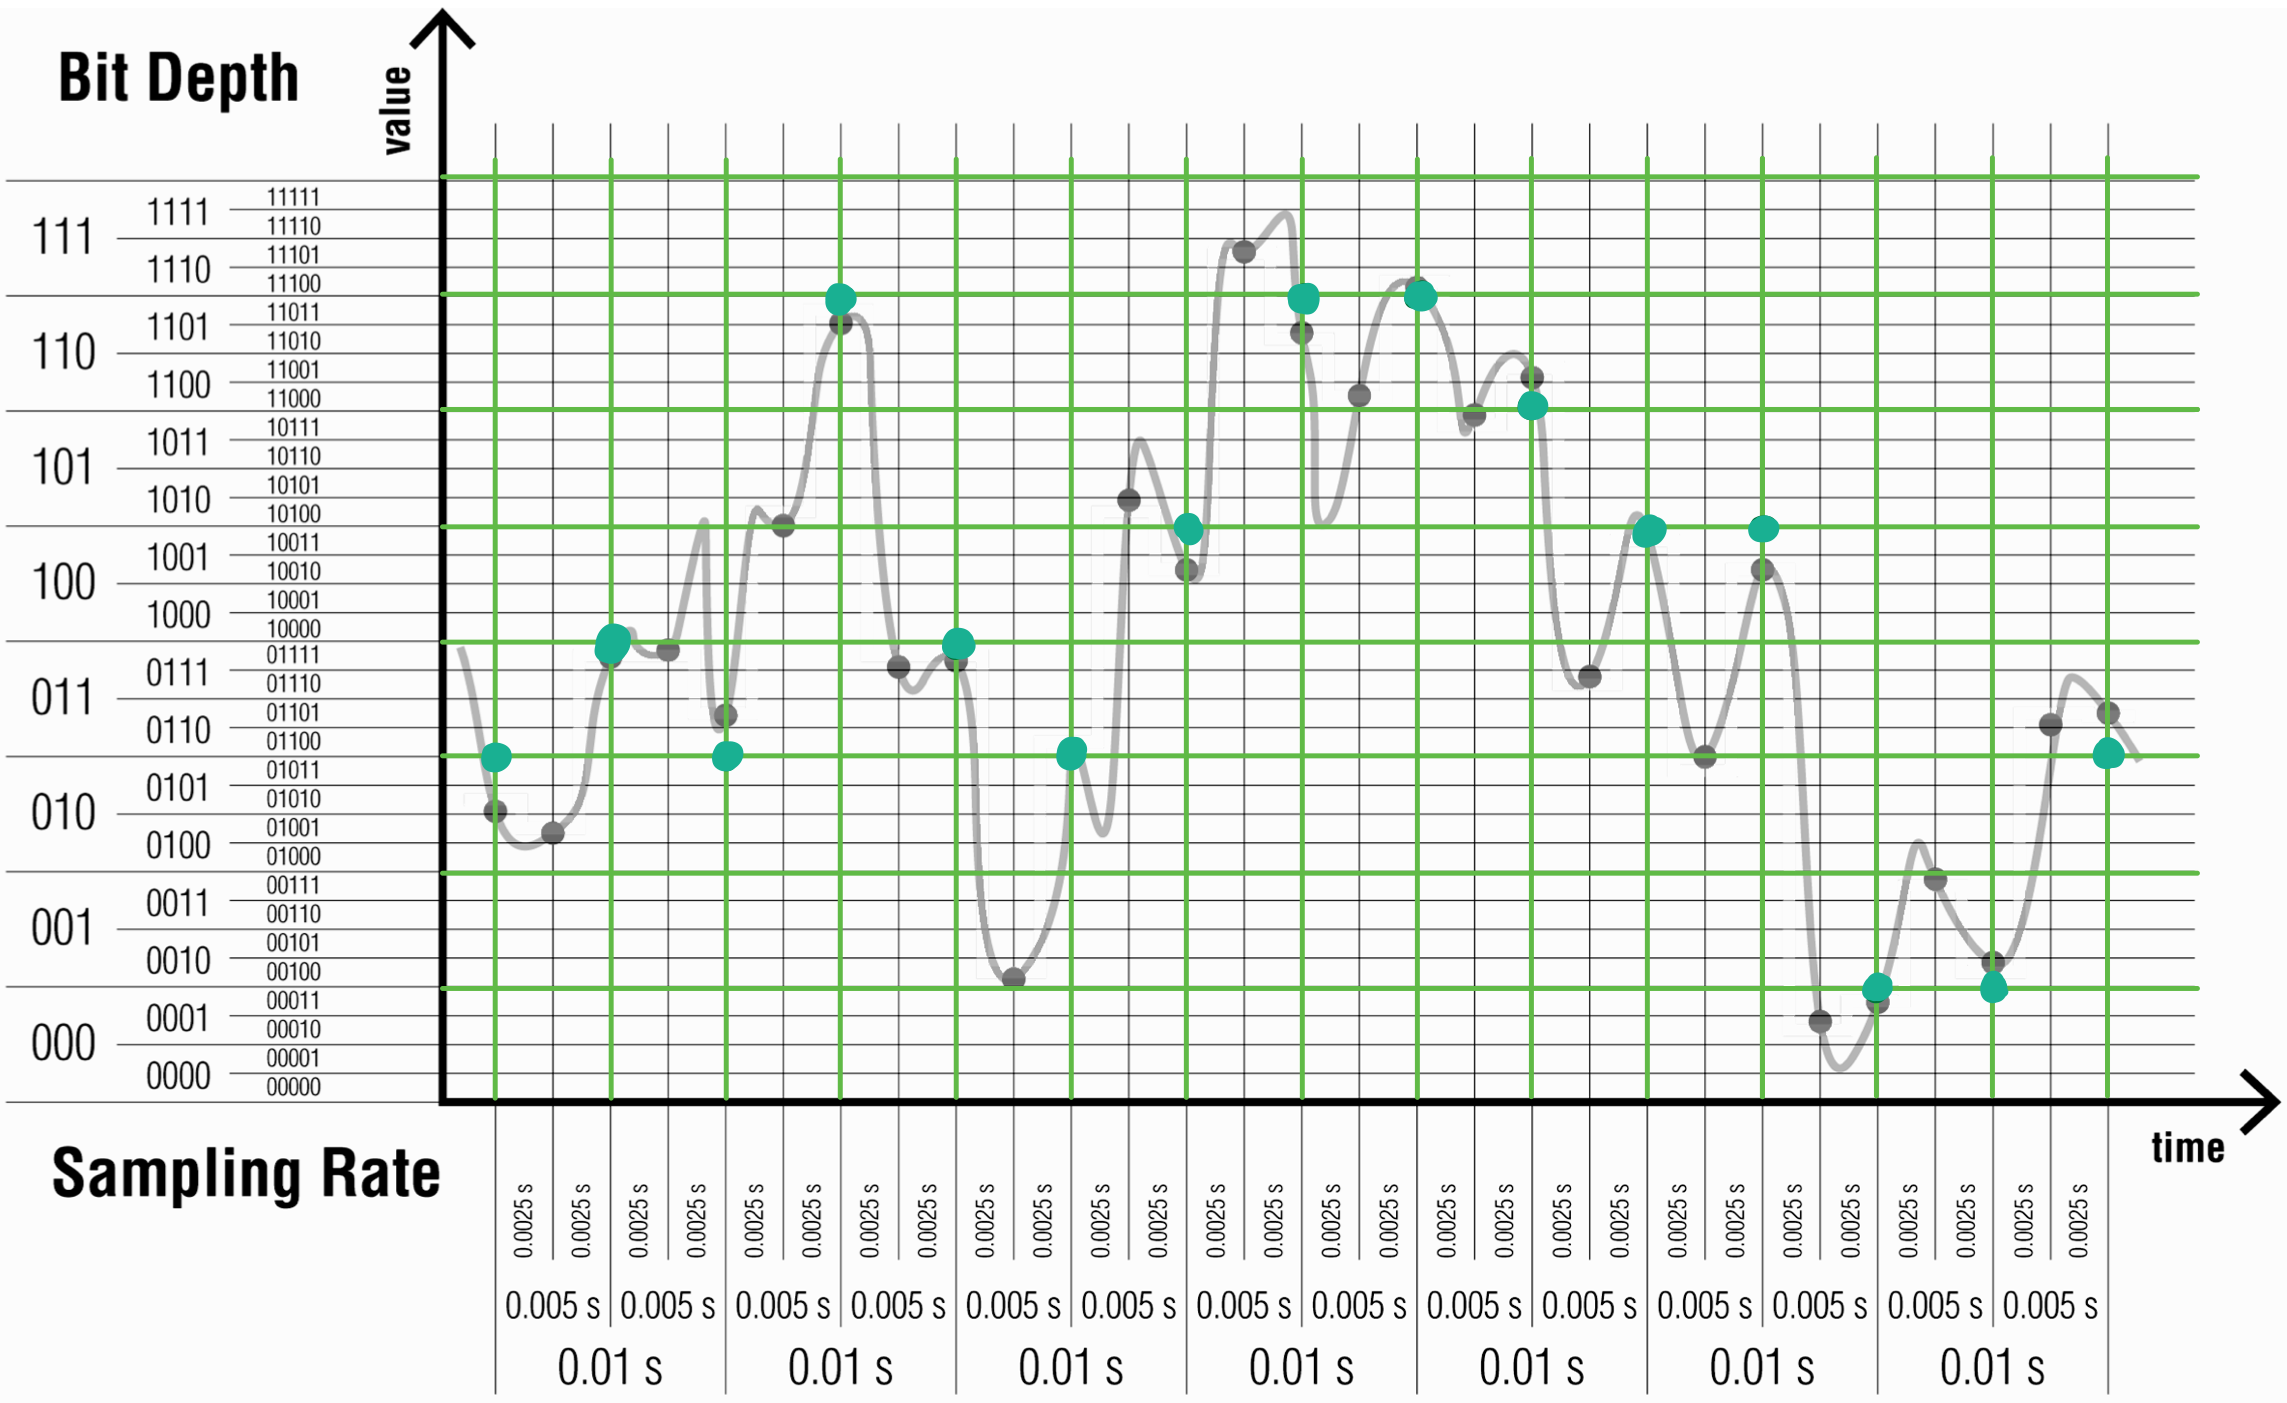
\includegraphics[width=1\linewidth]{solution-sampling-2.png}
	\end{figure}
\end{frame}

\lecture{Redondance}{week-13}

\subsection{Redondance}

\begin{frame}{Redondance : quésaco ?}{}
	Un des objectifs de l'ingénierie : construire des machines en lesquelles on peut avoir \textbf{confiance} (exemple de l'avion).
	\begin{itemize}
		\item <2-> Impossible d'éviter les soucis (hasard pas contrôlable, nature)
		\item <3-> Certains systèmes sont critiques (moteur de l'avion)
	\end{itemize}
	\uncover<4->{Il nous faut des solutions pour éviter les conséquences négatives (e.g. : éviter de mourir dès qu'un avion perd un moteur).}
\end{frame}

\begin{frame}{Redondance}{En informatique}
	Perte de données inévitable en informatique :
	\begin{itemize}
		\item <2-> \textbf{En transmission} : WiFi transmet dans l'air (murs, rebonds), câbles chauffent, etc.
		\item <3-> \textbf{Au stockage} : les disques durs vieillissent et causent des erreurs.
	\end{itemize}
\end{frame}

\begin{frame}{Redondance et résilience}{Note de vocabulaire}
	\begin{columns}
		\begin{column}{0.5\textwidth}
			\begin{definition}
				\textbf{Résilience} : capacité à se faire face, s'adapter et rebondir à moindre frais suite à un problème. \textbf{Notre but}.
			\end{definition}
		\end{column}
		\begin{column}{0.5\textwidth}
			\uncover<2->{\begin{definition}
					\textbf{Redondance} : duplication volontaire d'information ou de systèmes. \textbf{Moyen d'atteindre la résilience}, mais pas notre but premier (coûte cher !).
				\end{definition}}
		\end{column}
	\end{columns}
\end{frame}

\begin{frame}{Redondance}{Concrètement, comment faire ?}
	De nombreuses méthodes ! Voici l'une d'elles :
	\begin{definition}
		\textbf{Somme de contrôle/Checksum} : petite valeur à ajouter à un message qui permet de vérifier si une erreur est apparu dans ce dernier. Doit être \textbf{facile à calculer}, et \textbf{permet de détecter si un ou plusieurs bits sont erronés}.
	\end{definition}
\end{frame}

\begin{frame}{Somme de contrôle}{Le bit de parité}
	\begin{block}{Bit de parité}
		On fait la somme (décimale) des bits de la valeur à transmettre. Si cette somme est paire, on ajoute un 0 à droite, sinon on ajoute un 1 à droite et on transmet ce nouveau message.
	\end{block}

	\uncover<2->{\begin{exampleblock}{A la réception}
			En recevant le bloc de \textbf{9 bits}, on fait la somme des 8 premiers et on \textbf{vérifie} que si cette somme est paire, le bit le plus à droite est 0 et que sinon il est 1. Si ce n'est pas le cas, il y a eu une erreur lors de la transmissions !
		\end{exampleblock}}
\end{frame}

\begin{frame}{Somme de contrôle}{Le bit de parité}
	\begin{table}
		\begin{tabular}{|c|c|c|c|}
			\hline
			Bits à transmettre & Somme bits & Bit de parité & Bits transmis     \\ \hline
			0000000            & 0          & 0             & 0000000\textbf{0} \\ \hline
			0000001            & 1          & 1             & 0000001\textbf{1} \\ \hline
			0000010            & 1          & 1             & 0000010\textbf{1} \\ \hline
			0000011            & 2          & 0             & 0000011\textbf{0} \\ \hline
			0000100            & 1          & 1             & 0000100\textbf{1} \\ \hline
			%        0000101 & 2 & 0 & 0000101\textbf{0} \\ \hline
			%        0000110 & 2 & 0 & 0000110\textbf{0} \\ \hline
			%        0000111 & 3 & 1 & 0000111\textbf{1} \\ \hline
			…                  & ~          & …             & …                 \\ \hline
			1111101            & 6          & 0             & 1111101\textbf{0} \\ \hline
			1111110            & 6          & 0             & 1111110\textbf{0} \\ \hline
			1111111            & 7          & 1             & 1111111\textbf{1} \\ \hline
		\end{tabular}
	\end{table}
\end{frame}

\begin{frame}{Exercice}{Bit de parité}
	\begin{alertblock}{Exercice}
		Calculez le bit de parité de chacune des 3 lettres binaires (ASCII) que vous avez reçu. Sur une nouvelle feuille, recopiez la représentation binaire et ajoutez à droite le bit de parité. Si l’on vous indique d’insérer une erreur, inversez le bit indiqué (après avoir crée votre bit de parité) sur votre nouvelle feuille. Transmettez les chiffres binaires avec bit de parité à un.e voisin.e direct. Décidez si les messages que vous avez reçu contiennent une erreur.
	\end{alertblock}
\end{frame}

\begin{frame}{RAID}{Une autre technique de redondance}
	\begin{definition}
		Redundant Array of Independent Disks : procédé consistant à dupliquer en permanence toutes les données d'un disque sur un autre.
	\end{definition}

	\begin{exampleblock}{Simple mais efficace}
		Si l'un des disques a une panne, l'autre peut immédiatement prendre le relai et toutes les données sont toujours disponibles.
	\end{exampleblock}
\end{frame}

\begin{frame}{Conclusion du chapitre}{}
	\begin{itemize}
		\item On peut convertir des nombre en et depuis le binaire
		\item Représenter les nombres nous permet d'encoder des caractères ou des pixels de couleur
		\item Des techniques existent même pour encoder numériquement les ondes continues (avec des compromis)
		\item Ces données sont cruciales et on utilise des techniques pour s'assurer de leur bonne réception et lecture
	\end{itemize}
\end{frame}

\lecture{Algorithmes 1}{week-17}
\section{Algorithmique}

\begin{frame}{Algorithmes}{}
	\begin{columns}
		\begin{column}{0.7\textwidth}
			Quel est le programme ?
			\begin{itemize}
				\item \textbf{Quoi} ? Qu'est-ce qu'un algorithme ? Comment se différencie-t-il du programme ?
				\item<2-> \textbf{Pourquoi} ? Histoire très ancienne. Explosion depuis l'invention de machines !
				\item<3-> \textbf{Comment} ? Notion d'algorithme et solution aux problèmes. Comparaison de ces solution.
			\end{itemize}
		\end{column}
		\begin{column}{0.3\textwidth}
			\uncover<2->{
				\begin{figure}
					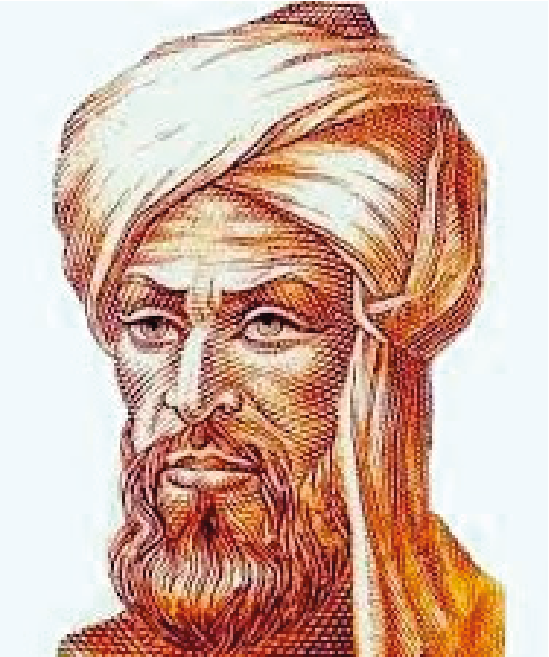
\includegraphics[width=1\linewidth]{Al-Khwarizmi.png}
					\caption{Considéré comme le père de l’algèbre Al-Khwarizmi a vécu au VIIIe siècle dans le Moyen-Orient.}
				\end{figure}
			}
		\end{column}
	\end{columns}

\end{frame}

\subsection{Les algorithmes}

\begin{frame}{Exercice : trouver le maximum}{}
	\begin{alertblock}{Exercice}
		10 cartes distribuées dans la classe, face cachée. Un·e élève doit venir au tableau et trouver le maximum parmi toutes les cartes. Seule ``opération'' autorisée est de demander à ses camarade un·e par un·e de montrer leur carte. Comment allez vous faire ?
	\end{alertblock}
	\pause
	\begin{exampleblock}{Solution}
		Il est possible de résoudre ceci avec un algorithme ! En quoi est-ce un algorithme ? Nous allons le voir.
	\end{exampleblock}
\end{frame}

\begin{frame}{Algorithmes}{Définitions}
	\begin{definition}
		\textbf{Algorithme} : procédure logique bien définie, étape par étape, pour résoudre un problème donné. \textbf{Destiné à des humains}
	\end{definition}

	\pause

	\begin{definition}
		\textbf{Programme} : ensemble d'instructions à suivre par un ordinateur. \textbf{Destiné à des machines}
	\end{definition}
\end{frame}

\begin{frame}{Algorithmes}{Structure d'un algorithme}
	\begin{figure}
		
\includegraphics[width=1\linewidth]{Diagramme_algorithme.png}
		\caption{Un algorithme est entièrement définit par ces 3 éléments}
	\end{figure}

	\pause
	\begin{columns}
		\begin{column}{0.33\textwidth}
			Utilise les données re\c cues en \textbf{entrée}.
		\end{column}
		\pause
		\begin{column}{0.33\textwidth}
			Effectue des \textbf{opérations} sur ces données.
		\end{column}
		\pause
		\begin{column}{0.33\textwidth}
			Retourne un \textbf{résultat} en sortie.
		\end{column}
	\end{columns}
\end{frame}

\begin{frame}{Exemple d'algorithme}{Recette de gâteau}
	\begin{algorithmic}[1]
		\REQUIRE 200g de farine; 2 œufs; 50g de beurre; 80g de sucre
		\pause
		\FORALL {$ingredient$}
		\pause
		\STATE mettre $ingredient$ dans un $plat$
		\pause
		\ENDFOR
		\State cuire $plat$ dans un four à 180° pendant 25mn
		\pause
		\ENSURE 1 gâteau
	\end{algorithmic}

\end{frame}

\begin{frame}{Algorithme du maximum}{Exercice}
	\begin{alertblock}{Construction de l'algorithme du maximum}
		Avec l'aide de votre voisin·e de table, définissez aussi \textbf{précisément que possible} les Données, Opérations et Sortie de l'algorithme employé par votre camarade en début de séance.
	\end{alertblock}
\end{frame}

\begin{frame}{Algorithme du maximum}{Solution}
	\begin{exampleblock}{Solution}
		\begin{algorithmic}[1]
			\REQUIRE
			La liste des valeurs des cartes tenues par vos camarades
			liste:=[3,19,4,21,11,20,4,17,3,1,1,4,10,16,18,2,8,6,16,15,2,21]
			\STATE $max\_actuel \gets 0$
			\FORALL{$nombre \in liste $}
			\IF{$nombre \geq max\_actuel$}
			\STATE $max\_actuel \gets nombre$
			\ENDIF
			\ENDFOR
			\RETURN $max\_actuel$
			\ENSURE Le plus grand nombre de la liste
		\end{algorithmic}
	\end{exampleblock}

\end{frame}

\begin{frame}{Simulation d'algorithmes}{Exercices}
	\begin{columns}
		\begin{column}{0.5\textwidth}
			\begin{alertblock}{Exercice}
				Suivez les instructions de l'exercice distribué
			\end{alertblock}
		\end{column}
		\begin{column}{0.5\textwidth}
			\begin{figure}
				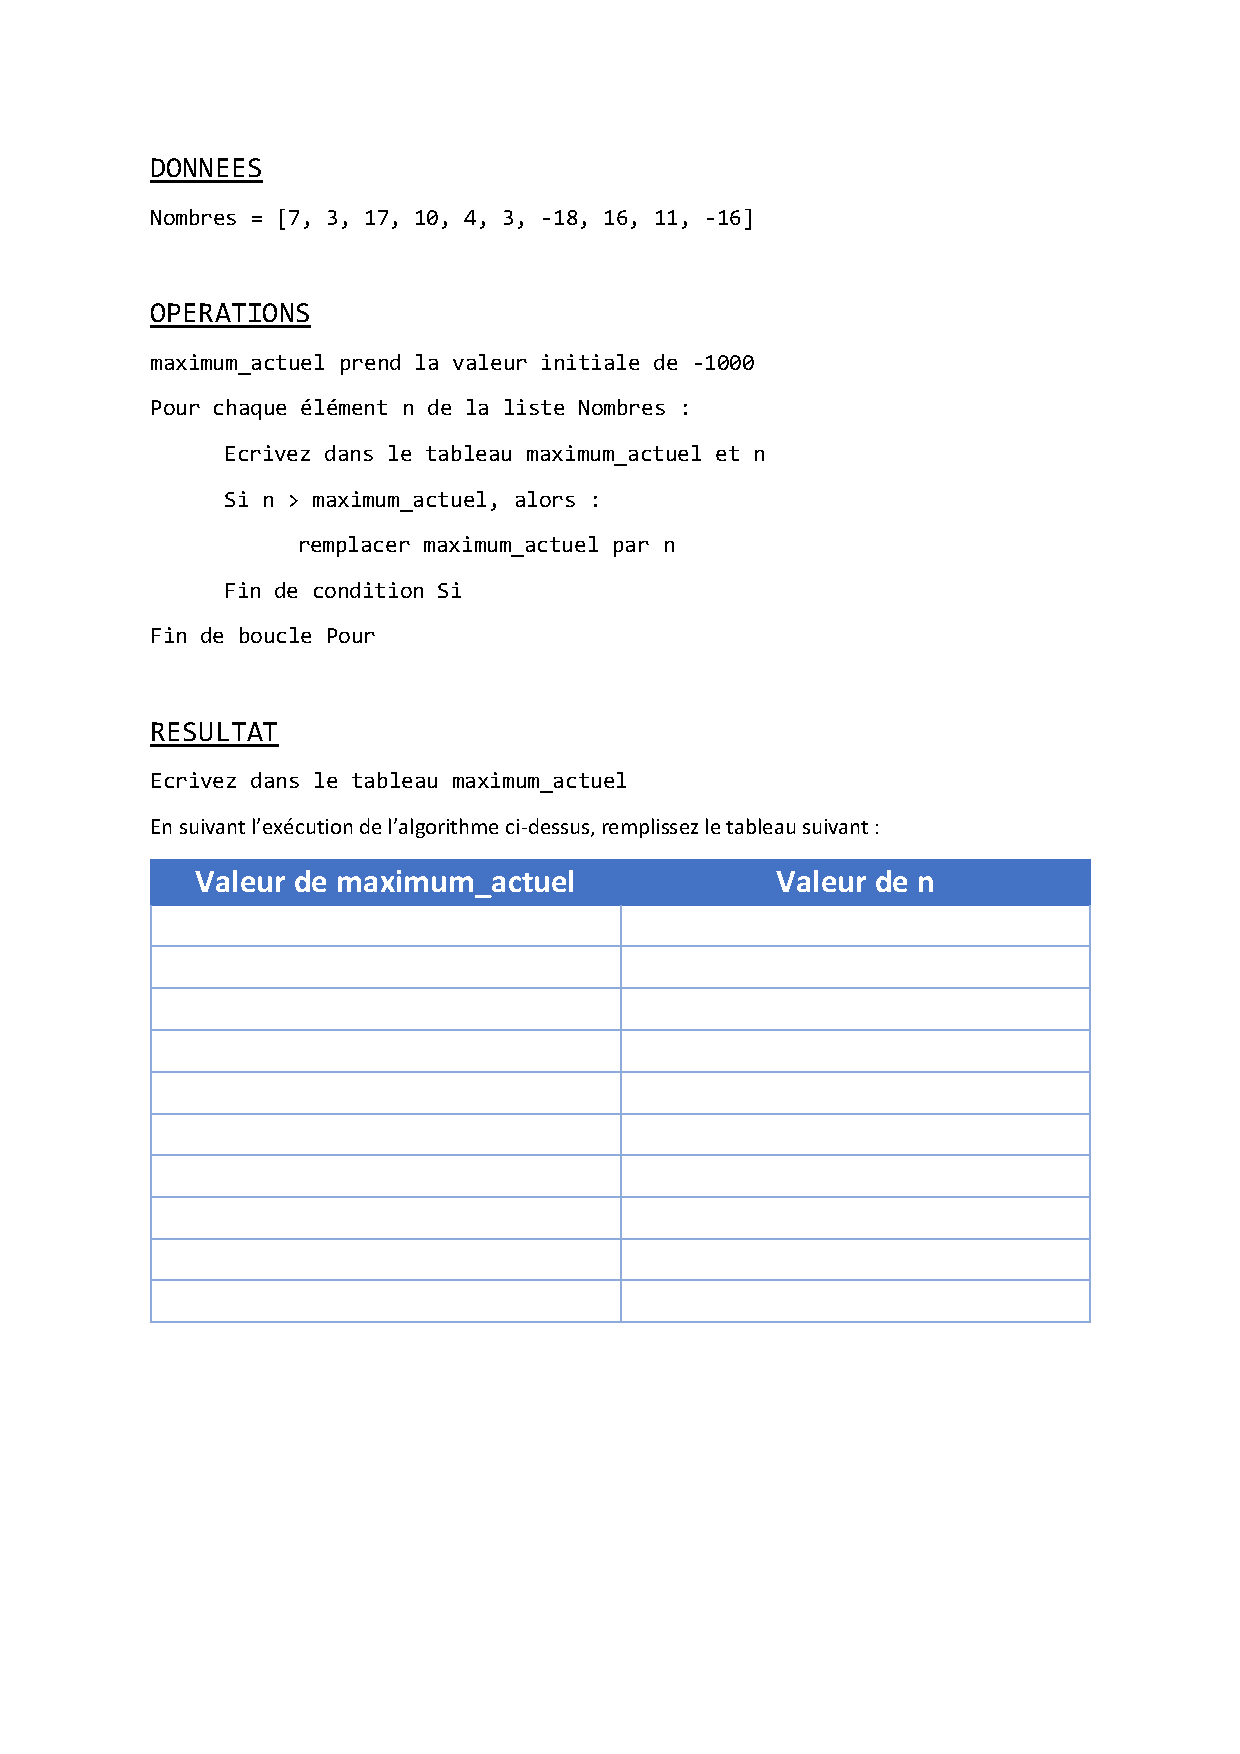
\includegraphics[width=1\linewidth]{ExerciceSimulationAlgorithme.pdf}
				\caption{Beamer presentation}
			\end{figure}
		\end{column}
	\end{columns}
\end{frame}

\begin{frame}{Algorithmes et informatique}{}
	\begin{figure}
		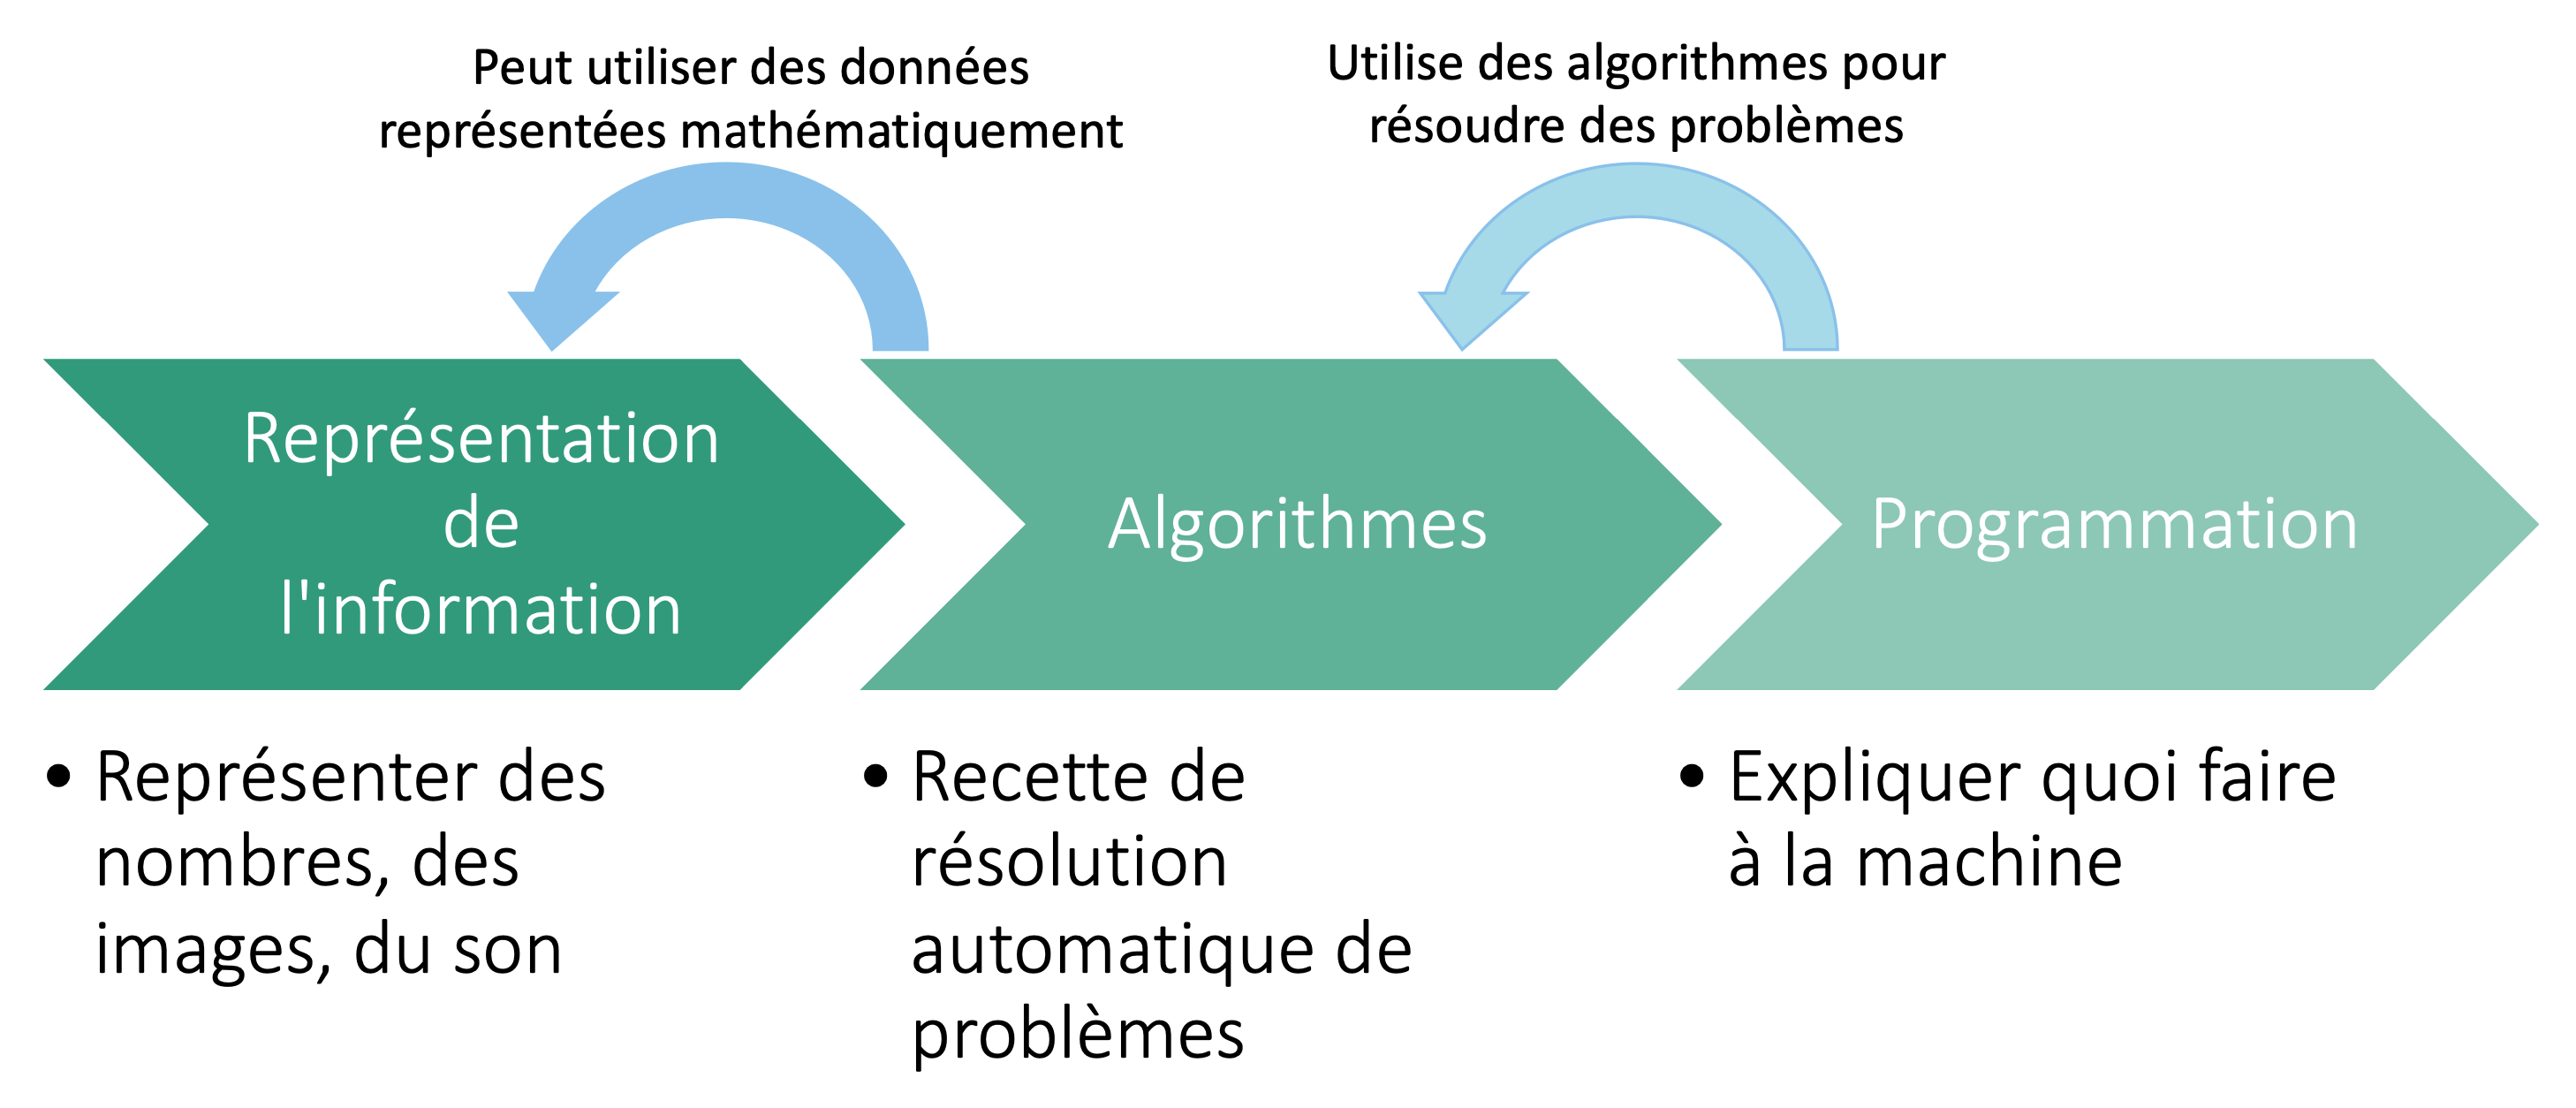
\includegraphics[width=1\linewidth]{algo_et_info.png}
	\end{figure}
\end{frame}

\lecture{Algorithmes : simulation et language}{week-18}

\begin{frame}{Le language des algorithmes}

	\begin{itemize}
		\item Algorithmes $\neq$ programmes
		\item<2-> Algorithmes pour les humains
		\item<3-> Syntaxe moins stricte ...
	\end{itemize}

\end{frame}

\begin{frame}{Le language des algorithmes}{Etre clair sans programmer}

	\begin{itemize}
		\item Pas de \texttt{SyntaxError}, contrairement à Python ! :)
		\item<2-> Mais attention : rester clair·e et \textbf{sans ambiguïté}
		\item<3-> \href{https://youtu.be/KY2z0YSw0Lk?t=12}{\beamergotobutton{``Exact instructions challenge''}}
		\item<4-> Algorithmes des slides $\rightarrow$ là pour vous guider
	\end{itemize}

\end{frame}

\begin{frame}{Algorithme mystère}{}

	\begin{algorithmic}[1]
		\REQUIRE Liste Nombres
		\STATE $n \gets longueur(Nombres)$
		\STATE $i \gets 1$
		\STATE $Resultat \gets 0$
		\FOR{$i \gets 1$ à $n$}
		\STATE $Resultat \gets Resultat + Nombres[i]$
		\ENDFOR
		\RETURN Résultat
		\ENSURE Résultat
	\end{algorithmic}

	%\begin{algorithmic}[1]
	%\REQUIRE Liste Nombres \COMMENT{la variable Nombres contient une liste de nombres}
	%\STATE $n \gets longueur(Nombres)$ \COMMENT{la variable n contient le nombre d'éléments dans Nombres}
	%\STATE $i \gets 1$ \COMMENT{la variable i contient 1 pour commencer}
	%\STATE $Resultat \gets 0$ \COMMENT{la variable Résultat contient 0 pour commencer}
	%\FOR{$i \gets 1$ à $n$} \COMMENT{i prend la valeur de 1, puis 2, puis 3, jusqu'à n}
	%	\STATE $Resultat \gets Resultat + Nombres[i]$ \COMMENT{Résultat vaut la somme de lui-même avec l'i-ème élément de Nombres}
	%\ENDFOR \COMMENT{quand i vaut n l'algorithme se termine}
	%\RETURN Résultat
	%\ENSURE Résultat
	%\end{algorithmic}

\end{frame}

\begin{frame}{Variables}{Une brique essentielle de nos algorithmes}
	\begin{columns}
		\begin{column}{0.6\textwidth}
			\begin{itemize}
				\item Variables = tiroirs avec étiquettes contenant des valeurs \pause
				\item Peuvent être modifiées, réutilisées \pause
				\item Un tiroir = une valeur = une étiquette \pause
			\end{itemize}
			\begin{exampleblock}{Exemple}
				Appelons une variable i. i peut contenir 1, puis contenir 2, mais pas 1 et 2 en même temps. i peut contenir \textbf{une} liste de valeurs [1,2] ou une autre liste [3,4], mais pas les deux en même temps.
			\end{exampleblock}
		\end{column}
		\begin{column}{0.4\textwidth}
			\begin{figure}
				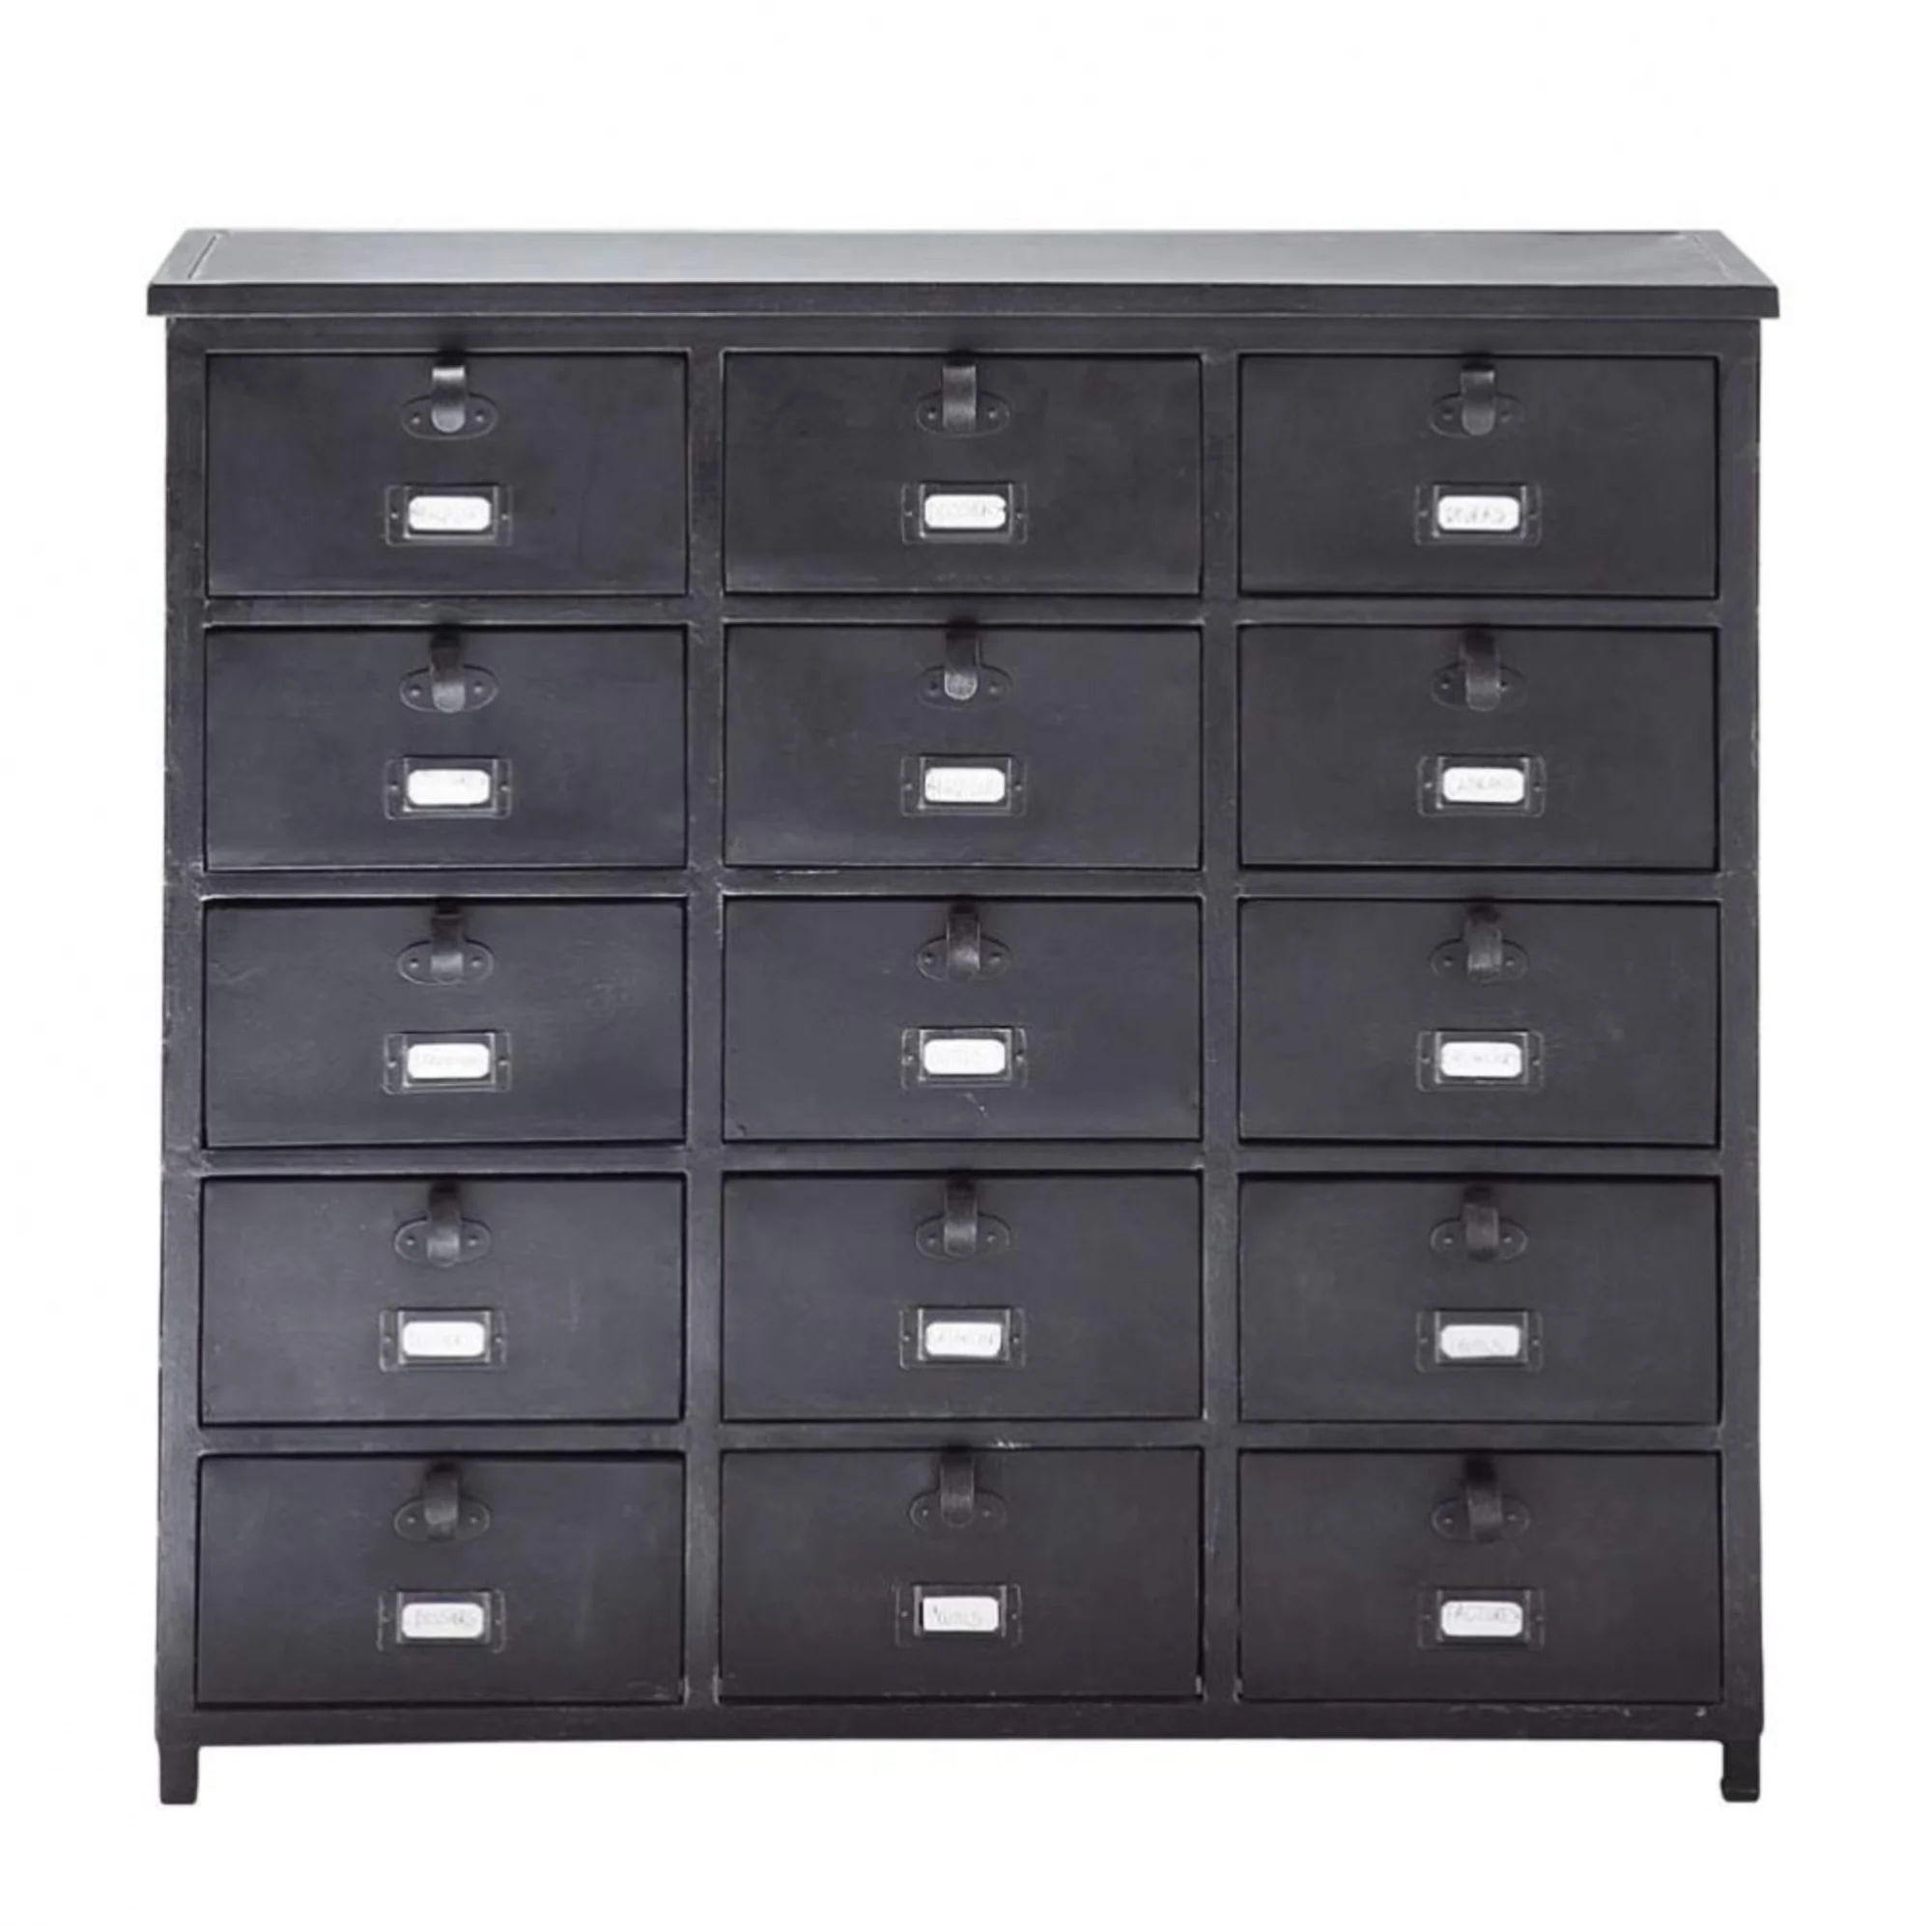
\includegraphics[width=1\linewidth]{Commode.png}
				\caption{Variables = tiroirs avec des étiquettes}
			\end{figure}
		\end{column}
	\end{columns}
\end{frame}

\begin{frame}{Simuler les algorithmes}{Comment simuler un algorithme ?}
	\begin{itemize}
		\item Pour simuler, besoin de valeurs \textbf{concrètes} dans les variables
		\item Exemple : La liste Nombres devient une vrai liste de nombres comme [1,4,7,23,6,1]
	\end{itemize}
\end{frame}

\begin{frame}{Simuler les algorithmes}{Retour sur l'algorithme mystère}
	\begin{algorithmic}[1]
		\REQUIRE Liste Nombres \COMMENT{la variable Nombres contient une liste de nombres} \pause
		\STATE $n \gets longueur(Nombres)$ \COMMENT{la variable n contient le nombre d'éléments dans Nombres} \pause
		\STATE $i \gets 1$ \COMMENT{la variable i contient 1 pour commencer} \pause
		\STATE $Resultat \gets 0$ \COMMENT{la variable Résultat contient 0 pour commencer} \pause
		\FOR{$i \gets 1$ à $n$} \COMMENT{i prend la valeur de 1, puis 2, puis 3, jusqu'à n} \pause
		\STATE $Resultat \gets Resultat + Nombres[i]$ \COMMENT{Résultat vaut la somme de lui-même avec l'i-ème élément de Nombres} \pause
		\ENDFOR \COMMENT{quand i vaut n l'algorithme se termine} \pause
		\ENSURE Résultat
	\end{algorithmic}
\end{frame}

\begin{frame}{Simuler les algorithmes}{Des tiroirs aux tableaux}
	\begin{itemize}
		\item En test : pas de tiroirs \pause
		\item Tableau : voir les différentes valeurs des variables
	\end{itemize}
	\begin{table}[!ht]
		\centering
		\begin{tabular}{c|c|c|c}
			\hline
			\textbf{Passage dans la boucle} & \textbf{i} & \textbf{Nombres[i]} & \textbf{Résultat} \\ \hline  \pause
			avant                           & 1          & 4                   & 0                 \\ \hline \pause
			1                               & 1          & 4                   & 4                 \\ \hline \pause
			2                               & 2          & 5                   & 9                 \\ \hline \pause
			3                               & 3          & 6                   & \textbf{15}       \\ \hline
		\end{tabular}
	\end{table}
\end{frame}

\begin{frame}{Simuler les algorithmes}{Que fait l'algorithme mystère ?}
	\begin{columns}
		\begin{column}{0.7\textwidth}
			\begin{itemize}
				\item ? \pause
				\item Somme de tous les nombres d'une liste ! \pause
				\item Rapport avec une utilité concrète ? \pause
				\item Caisse enregistreuse !
			\end{itemize}
		\end{column}
		\begin{column}{0.3\textwidth}
			\begin{figure}
				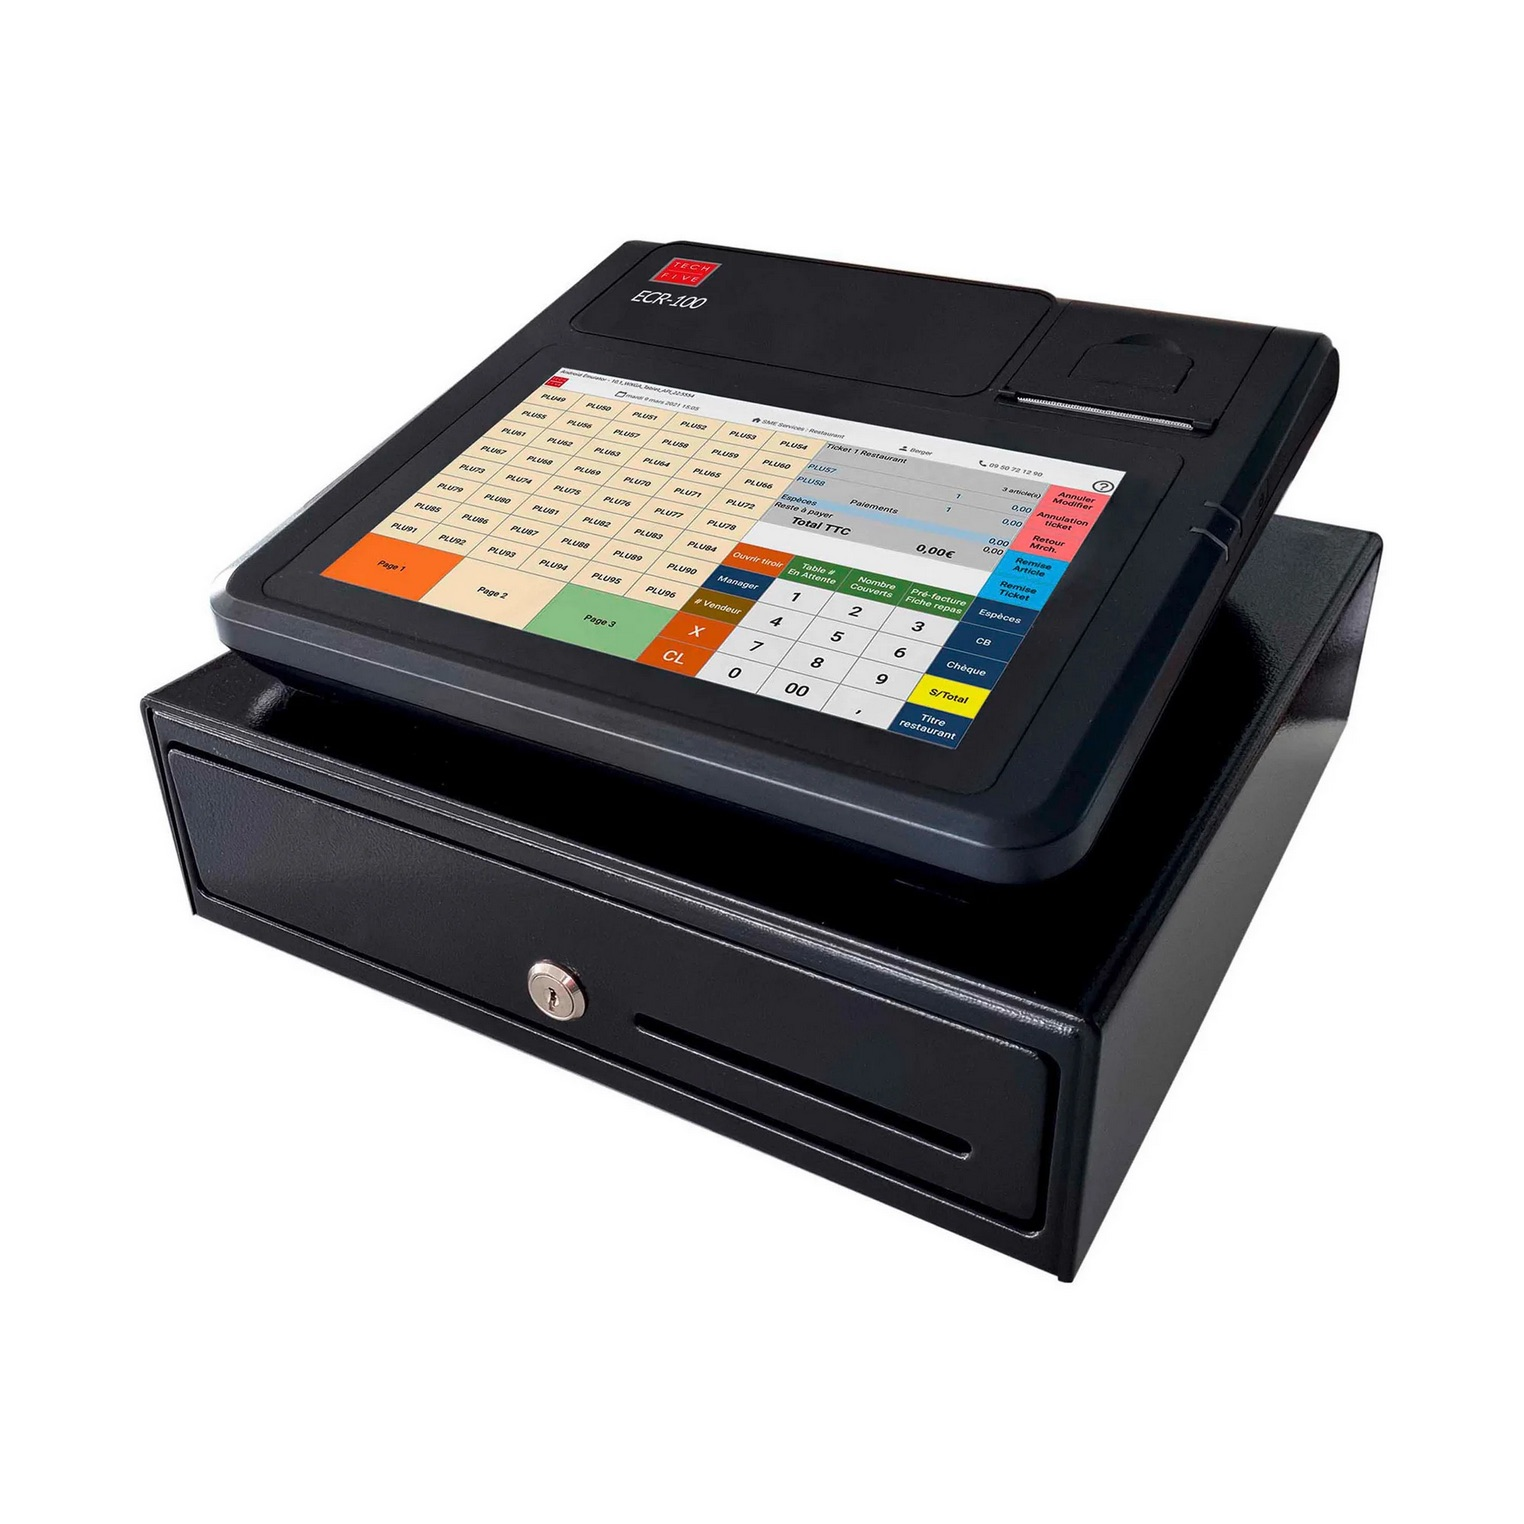
\includegraphics[width=1\linewidth]{caisse.jpeg}
			\end{figure}
		\end{column}
	\end{columns}
\end{frame}

\begin{frame}{Exercices}{Simulation d'algorithmes}
	\begin{alertblock}{Forme mystère}
		L’algorithme suivant contrôle un crayon. Quelle forme dessine-t-il ?
		\begin{algorithmic}[1]
			\REPEAT
			\STATE Avance de 2cm
			\STATE Tourne à droite de 60°
			\UNTIL{a été répété 8 fois}
		\end{algorithmic}
	\end{alertblock}
\end{frame}

\begin{frame}{Exercices}{Simulation d'algorithmes}
	\begin{alertblock}{Echange de 2 variables}
		Écrire un algorithme qui échange les valeurs de deux variables. Par exemple, si la première variable X contient 1 et la deuxième variable Y contient 2, à la fin de l’algorithme X contient 2 et Y contient 1. Pour rappel, une variable peut contenir une seule valeur à la fois.
	\end{alertblock}
	\begin{exampleblock}{Conseil}
		Cela aide de se mettre à la place de la machine et de représenter le contenu de chaque variable sous la forme d’un tiroir, en la dessinant avec son étiquette et son contenu après chaque opération de votre algorithme.
	\end{exampleblock}
\end{frame}

\begin{frame}{Exercices}{Simulation d'algorithmes}
	\begin{alertblock}{Affectations}
		Quel est le résultat de la suite des trois affectations suivantes ?

		Vérifier votre solution en représentant chaque variable et en y mettant des valeurs fictives. Suivre les opérations dans l’ordre et dessiner le contenu des variables après chaque étape.
		\begin{algorithmic}[1]
			\REQUIRE 2 variables X et Y, contenant chacune une valeur
			\STATE $X \gets X+Y$
			\STATE $Y \gets X-Y$
			\STATE $X \gets X-Y$
		\end{algorithmic}
	\end{alertblock}
\end{frame}

\lecture{}{}

\subsection{Trie, cherche et trouve}

\subsection{Des algorithmes aux programmes}

\section{Programmation}
\section{Architecture des ordinateurs}
\section{Enjeux sociaux de l'informatique}

\lecture{Uberisation 1}{week-14}

\begin{frame}{Enjeux sociaux}{}
	Le numérique nous apporte beaucoup de questionnements, problèmes et solutions techniques ! Qu'en est-il des conséquences sociales ?
	\begin{block}{Objectif}
		Apporter des informations et des questionnement pour permettre une meilleure discussion sur ces enjeux. Certains concepts sont à connaître et des outils nous permettrons de mieux comprendre certaines situations !
	\end{block}
\end{frame}

\subsection{Économie du numérique}

\begin{frame}{Le numérique au coeur de l'économie moderne}{Raisons et risques}
	\begin{itemize}
		\item Quelles sont les logiques d’expansion des plateformes numériques ?
		\item En quoi l’acronyme GAFAM est-il pertinent ?
		\item Que nous apprend le concept d’économie de l’attention ?
	\end{itemize}
\end{frame}

\begin{frame}{Logiques d'expansion des plateformes numériques}{Vocabulaire}
	\begin{itemize}
		\item \textbf{Effet de réseau} : plus il y d'utilisateur.trice.s, plus d'utilisateur.trice.s sont attiré.e.s (Instagram, BeReal, intéressant quand beaucoup de nos ami.e.s y sont).
		\item<2-> \textbf{Economies d'échelle} : la production d'un produit peut coûter cher, mais une fois l'investissement fait, produire un deuxième coûte moins cher (production de téléphone demande une usine, une fois l'usine en place on peut produire beaucoup de téléphone).
		\item<3-> \textbf{Logique du ``winner takes it all''} : système qui, par nature, a tendance à favoriser le monopole économique (Amazon est pratique car il y a un seul endroit pour tout trouver).
	\end{itemize}
\end{frame}

\begin{frame}{Logiques d'expansion des plateformes numériques}{Vocabulaire}
	\begin{itemize}
		\item \textbf{Uberisation}
		      \begin{itemize}
			      \item Contourner le fonctionnement classique en créant un nouvel intermédiaire via une plateforme numérique
			      \item Relation client-prestataire avec commission
			      \item Flexible, moins cher, mais stratégie agressive et obscure
		      \end{itemize}
	\end{itemize}

	\href{https://www.youtube.com/watch?v=ST_KVB6bEdw}{\beamergotobutton{click here}}
\end{frame}

\begin{frame}{Uberisation}{Questions}
	\begin{itemize}
		\item Présentez en quelques mots le modèle économique de Uber Eats.
		\item En quoi le modèle économique de Uber Eats n’est-il pas soutenable pour les livreurs?
		\item Quelles sont les données produites par les livreurs et en quoi sont-elles utiles à Uber?
		\item Livreurs, restaurants et particuliers sont notés : quel est l’objectif de ces évaluations?
		\item Peut-on dire qu’Uber propose une technologie ``innovante''?
	\end{itemize}
\end{frame}

\lecture{Uberisation 2}{week-15}

\begin{frame}{Uberisation}{Eléments de réponses}
	\begin{itemize}
		\item<1-> Service de livraison de repas
		\item<2-> Salaire insuffisant; désavantages d'entrepreneur.euse et de salarié.e (temps d'attente pas payé, pas de prestations sociales, exigences de la plateformes)
		\item<3-> Connecté à l'application pour travailler : envoi de localisation, vitesse, profil (étoiles et score), clients : permet d'analyser et optimiser (valoriser rapides, sanctionner les moins rapides).
		\item<4-> Notation permet d'optimiser les flux et d'avoir un moyen de pression sur les livreur.euse.s. Pas objectif ! (dépend du contexte émotionnel des client.e.s).
		\item<5-> Innovation : algorithme puissant, mais application de commandes de taxi existaient déjà ! Innovation technologique ou stratégique ?
	\end{itemize}
\end{frame}

\begin{frame}{Uberisation}{Lecture de l'article de Le Temps}
	\begin{itemize}
		\item Résumez l’article en une phrase.
		\item Expliquez l’importance de cette nouvelle.
		\item Quelles peuvent-être les conséquences de ce changement de politique?
		\item Quel sens donner au mot ``flexibilité'' du porte-parole d’Uber ?
	\end{itemize}
\end{frame}

\begin{frame}{Uberisation}{Eléments de réponse}
	\begin{itemize}
		\item<1-> Livreur.euse.s sont des employé.e.s de Uber : salaire, cotisation, chômage
		\item<2-> D'autres États pourraient suivre ceci. Uber peut-il s'adapter et payer un salaire minimum aux livreur.euse.s ? Conséquences sur les prix des courses.
		\item<3-> Flexibilité permet de choisir ses horaires de travail. Cache une grande précarité : pas de revenus garantis, moins d'activité est sanctionné indirectement. Profite à l'employeur.euse ou l'employé.e ? Pas de responsabilités pour Uber (maladies, accidents, baisse des commandes) ! Importation du système Uber dans le monde : vision qui ne convient pas à tout le monde, besoin d'adaptations.
	\end{itemize}
\end{frame}

\lecture{Enchères du web}{week-16}

\begin{frame}{Enchères du web}{Monopoly 2.0}
	Données personnelles vendues pour la \textbf{publicité ciblée}. Concrètement, comment ça se passe ?
\end{frame}

\begin{frame}{Enchères du web}{Présentation du jeu}
	\begin{exampleblock}{Instruction}
		Répartition en 4 groupes d'annonceur.euse.s
	\end{exampleblock}
	\begin{figure}
		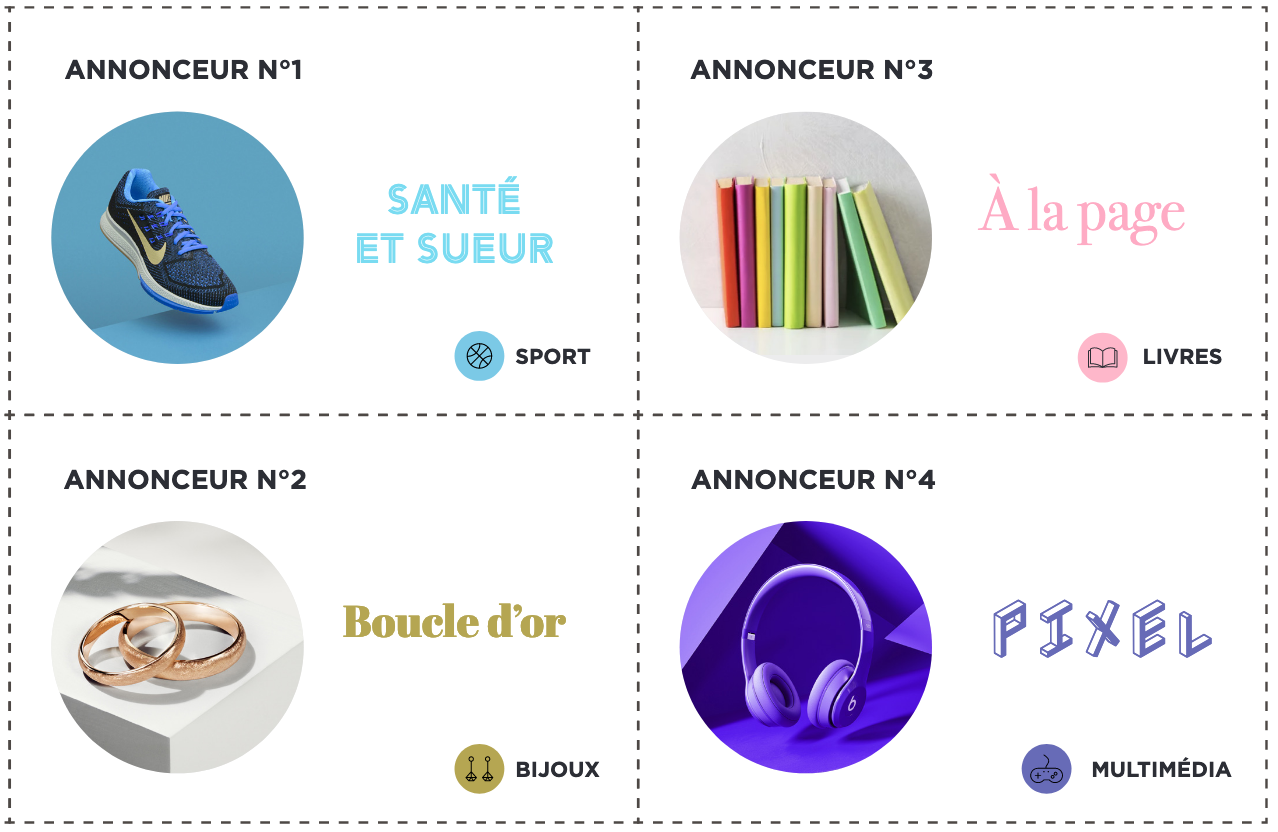
\includegraphics[width=0.5\linewidth]{annonceurs.png}
		\caption{Les annonceur.euse.s de notre plateforme}
	\end{figure}
\end{frame}

\begin{frame}{Enchères du web}{Présentation du jeu}
	\begin{exampleblock}{Instruction}
		Un papier et un crayon à papier par groupe pour annoncer la valeur misée.
	\end{exampleblock}
	\uncover<2->{\begin{alertblock}{Objectif}
			Le groupe rapportant le plus d'argent après le dernier visiteur remportera le jeu.
		\end{alertblock}}
	\uncover<3->{\begin{block}{Comment gagner ?}
		Je suis une plateforme en ligne et vous propose de montrer vos annonces à des client.e.s potentiels qui achèteront vos produits.}
	\end{block}
\end{frame}

\begin{frame}{Enchères du web}{Présentation du jeu}
	\begin{block}{Tour d'achat}
		\begin{itemize}
			\item<1-> Un.e client arrive : votre groupe discutez d'un prix à payer pour votre annonce
			\item<2-> Le groupe avec le plus gros prix gagne, et paye le prix proposé par le groupe avec le \textbf{second plus gros prix}
			\item<3-> Le groupe gagnant tente de vendre \textbf{5 produits} au/à la client.e
		\end{itemize}
	\end{block}

\end{frame}

\begin{frame}{Enchères du web}{Présentation du jeu}
	\begin{block}{Caractéristiques des client.e.s}
		\begin{itemize}
			\item Achète un produit si le \textbf{lancé de dés est suffisamment haut}
			\item<2-> 50\% de chance d'être intéressé.e par votre produit (dépend des client.e.s)
			\item<3-> Si intéressé.e, rapporte en moyenne entre 70CHF et 90CHF
			\item<4-> Si pas intéressé.e, rapport en moyenne entre 10CHF et 30CHF
		\end{itemize}
	\end{block}
\end{frame}

\begin{frame}{Enchères du web}{Première enchère}

\end{frame}

\begin{frame}{Enchères du web}{Conclusion}
	\begin{itemize}
		\item Fonctionnement réel ! (automatisé et en quelques millisecondes)
		\item<2-> \href{https://fr.wikipedia.org/wiki/William_Vickrey}{\beamergotobutton{Enchères de Vickrey}}
		\item<3-> Compétition entre les vendeurs, prise de risque, probabilité de gain
		\item<4-> Google a réalisé 61 milliards de bénéfice en 2021 avec la publicité
		\item<5-> Tournant du jeu : information sur les client.e.s !
		\item<6-> Quelles limites ?
	\end{itemize}
\end{frame}

\lecture{}{}

\subsection{Vie privée et surveillance}

\subsection{Les femmes dans l'histoire de l'informatique}

\end{document}
